\documentclass[journal]{IEEEtran}
\usepackage{cite}
\usepackage{amsmath,amssymb,amsfonts}
\usepackage{algorithm}
\usepackage{algpseudocode}
\usepackage{graphicx}
\usepackage{textcomp}
\usepackage{booktabs}
\usepackage{multirow}
\usepackage{tikz}
\usepackage{pgfplots}
\pgfplotsset{compat=1.18}
\usetikzlibrary{arrows.meta,positioning,shapes.geometric,calc,backgrounds,fit}

\newtheorem{theorem}{Theorem}
\newtheorem{proposition}{Proposition}
\newtheorem{definition}{Definition}
\newtheorem{assumption}{Assumption}

\begin{document}

\title{POLARIS: Polar-Oriented Layered Antipodal Riemannian Isometric Sphere for Joint Lexical Polarity and Document Representation Learning}

\author{Mohamed S. Amer and Ahmed B. Zaky%
\thanks{Manuscript received October 2026.}%
\thanks{Mohamed S. Amer and Ahmed B. Zaky are with the Department of Computer Science and Engineering, Egypt-Japan University of Science and Technology (E-JUST), New Borg El-Arab City, Alexandria 21934, Egypt (e-mail: mohamed.320230188@ejust.edu.eg; ahmed.zaky@ejust.edu.eg).}}

\maketitle

\begin{abstract}
Spherical text embedding models map words and documents onto the unit hypersphere $\mathbb{S}^{p-1}$ to align representation learning with directional cosine similarity. However, existing single-layer spherical formulations collapse synonyms and antonyms into overlapping neighborhoods near the same polar cap because opposite words share identical distributional contexts. When directional objectives optimize co-occurrence probabilities alone, antithetical concepts such as \textit{good} and \textit{bad} or \textit{win} and \textit{lose} converge toward positive cosine similarity, degrading both lexical similarity benchmarks and sentiment-sensitive document representations. To resolve this geometric collapse, we propose POLARIS (Polar-Oriented Layered Antipodal Riemannian Isometric Sphere), a multi-layer Riemannian representation framework on $\mathbb{S}^{99}$ ($p=100$) that partitions the unit hypersphere into three distinct functional zones: a North Polar Cap ($\cos\theta\to+1.0$) for synonyms and co-occurring terms, an Equatorial Orthogonality Belt ($\cos\theta\to0.0$) for unrelated negative samples to suppress high-dimensional hubness, and a South Antipodal Pole ($\cos\theta\to-1.0$) for lexical antonyms. POLARIS constructs $L=3$ concentric spherical layers coupled by chains of norm-preserving $\mathcal{O}(p)$ Householder reflections, a self-calibrating monotonic concentration cascade ($\kappa^{(1)}>\kappa^{(2)}>\kappa^{(3)}>2.0$), two-hop signed geodesic involution over lexical graphs, bipartite word-document-word tangent bundle transport, and idiom-protected spherical negation reflection. We establish finite-horizon Riemannian descent guarantees alongside asymptotic Robbins-Siegmund stationarity conditions for our tangential geodesic optimizer. Evaluated across 10 independent random seeds on SimLex-999, WordNet, 20 Newsgroups, and Rotten Tomatoes reviews using paired Student's $t$-tests with Holm-Bonferroni correction, POLARIS raises held-out antonym-synonym AUC from $0.5280$ to $0.9886$, reduces Antipodal Alignment Score from $1.4568$ to $0.6108$, improves SimLex-999 Spearman $\rho$ from $0.121$ to $0.435$, and boosts 20 Newsgroups Macro-F1 from $0.329$ to $0.467$.
\end{abstract}

\begin{IEEEkeywords}
Antipodal geometry, Householder reflections, lexical polarity, Riemannian optimization, spherical embeddings, text clustering, von Mises-Fisher distribution.
\end{IEEEkeywords}

% === SECTION I: INTRODUCTION ===
\section{Introduction}
\IEEEPARstart{D}{irectional} similarity metrics, particularly cosine similarity $\cos(\mathbf{u}, \mathbf{v}) = \mathbf{u}^\top \mathbf{v} / (\|\mathbf{u}\|_2 \|\mathbf{v}\|_2)$, govern information retrieval, document clustering, and semantic similarity evaluation, yet standard word and paragraph embedding models train in unconstrained Euclidean space $\mathbb{R}^p$ before applying post-hoc $\ell_2$ projection onto the unit hypersphere $\mathbb{S}^{p-1}$ \cite{mikolov2013distributed,pennington2014glove,meng2019spherical}. Projecting Euclidean vectors onto $\mathbb{S}^{p-1}$ after training introduces distortion because radial vector norms absorb frequency artifacts during optimization, causing angular distances on the sphere to diverge from the inner-product geometry optimized during training \cite{meng2019spherical,banerjee2005clustering}. Joint Spherical Embedding (JoSE) \cite{meng2019spherical} addressed this metric mismatch by formulating word-word and word-document co-occurrence directly on $\mathbb{S}^{p-1}$ using Riemannian gradient descent and von Mises-Fisher (vMF) directional distributions. Despite resolving the Euclidean-to-spherical projection mismatch, single-layer directional models exhibit a structural failure mode when representing semantic opposition: they cannot distinguish synonyms from antonyms.

\begin{figure*}[!t]
\centering
\resizebox{\textwidth}{!}{%
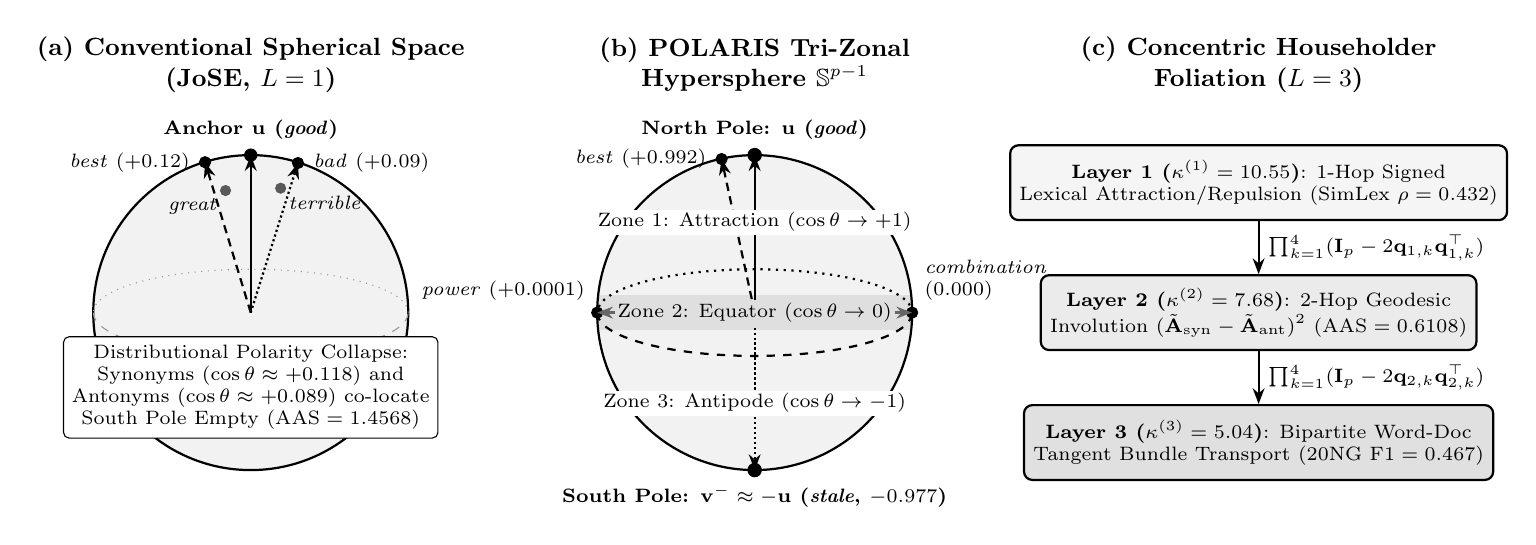
\begin{tikzpicture}[every node/.style={font=\footnotesize, text=black}]
% Left Panel: Collapse in Standard Spherical Embeddings (JoSE)
\begin{scope}[shift={(-6.4,0)}]
    \node[font=\bfseries\small, align=center] at (0, 3.15) {(a) Conventional Spherical Space\\(JoSE, $L=1$)};
    \fill[gray!10] (0,0) circle (2.0cm);
    \draw[thick, black] (0,0) circle (2.0cm);
    \draw[dashed, gray!80] (-2.0,0) arc (180:360:2.0cm and 0.55cm);
    \draw[dotted, gray!80] (2.0,0) arc (0:180:2.0cm and 0.55cm);
    
    % North Pole Collapse
    \filldraw[black] (0, 2.0) circle (2.2pt) node[above=2pt, font=\bfseries\scriptsize] {Anchor $\mathbf{u}$ (\textit{good})};
    \filldraw[black] (-0.58, 1.91) circle (2.0pt) node[left=2pt, font=\scriptsize] {\textit{best} ($+0.12$)};
    \filldraw[black] (0.60, 1.90) circle (2.0pt) node[right=2pt, font=\scriptsize] {\textit{bad} ($+0.09$)};
    \filldraw[gray!70!black] (-0.32, 1.55) circle (1.8pt) node[below left=-1pt, font=\scriptsize] {\textit{great}};
    \filldraw[gray!70!black] (0.38, 1.58) circle (1.8pt) node[below right=-1pt, font=\scriptsize] {\textit{terrible}};
    
    \draw[-{Stealth[length=2mm]}, thick, black] (0,0) -- (0,2.0);
    \draw[-{Stealth[length=2mm]}, thick, black, densely dashed] (0,0) -- (-0.58,1.91);
    \draw[-{Stealth[length=2mm]}, thick, black, densely dotted] (0,0) -- (0.60,1.90);
    
    \node[align=center, fill=white, draw=black, rounded corners=2pt, inner sep=3pt, font=\scriptsize] at (0, -0.95) {Distributional Polarity Collapse:\\Synonyms ($\cos\theta \approx +0.118$) and\\Antonyms ($\cos\theta \approx +0.089$) co-locate\\South Pole Empty ($\text{AAS} = 1.4568$)};
\end{scope}

% Center Panel: POLARIS Tri-Zonal Geometry
\begin{scope}[shift={(0.0,0)}]
    \node[font=\bfseries\small, align=center] at (0, 3.15) {(b) POLARIS Tri-Zonal\\Hypersphere $\mathbb{S}^{p-1}$};
    \fill[gray!10] (0,0) circle (2.0cm);
    \fill[gray!25] (-2.0, -0.22) rectangle (2.0, 0.22);
    \draw[thick, black] (0,0) circle (2.0cm);
    \draw[thick, black, dashed] (-2.0,0) arc (180:360:2.0cm and 0.55cm);
    \draw[thick, black, dotted] (2.0,0) arc (0:180:2.0cm and 0.55cm);
    
    % North Pole Zone
    \filldraw[black] (0, 2.0) circle (2.4pt) node[above=2pt, font=\bfseries\scriptsize] {North Pole: $\mathbf{u}$ (\textit{good})};
    \filldraw[black] (-0.42, 1.95) circle (2.0pt) node[left=2pt, font=\scriptsize] {\textit{best} ($+0.992$)};
    \draw[-{Stealth[length=2mm]}, thick, black] (0,0) -- (0,2.0);
    \draw[-{Stealth[length=2mm]}, thick, black, densely dashed] (0,0) -- (-0.42,1.95);
    
    % Equatorial Zone (multi-line label avoids collision with panel c)
    \filldraw[black] (2.0, 0) circle (2.0pt) node[above right=1pt and 1pt, align=left, font=\scriptsize] {\textit{combination}\\($0.000$)};
    \filldraw[black] (-2.0, 0) circle (2.0pt) node[above left=1pt and 1pt, align=right, font=\scriptsize] {\textit{power} ($+0.0001$)};
    \draw[-{Stealth[length=2mm]}, thick, gray!80!black] (0,0) -- (2.0,0);
    \draw[-{Stealth[length=2mm]}, thick, gray!80!black] (0,0) -- (-2.0,0);
    
    % South Pole Antipodal Zone
    \filldraw[black] (0, -2.0) circle (2.4pt) node[below=2pt, font=\bfseries\scriptsize] {South Pole: $\mathbf{v}^- \approx -\mathbf{u}$ (\textit{stale}, $-0.977$)};
    \draw[-{Stealth[length=2mm]}, thick, black, densely dotted] (0,0) -- (0,-2.0);
    
    % Labels for Zones
    \node[font=\scriptsize, fill=white, inner sep=1pt] at (0, 1.15) {Zone 1: Attraction ($\cos\theta \to +1$)};
    \node[font=\scriptsize, fill=gray!25, inner sep=1pt] at (0, 0.0) {Zone 2: Equator ($\cos\theta \to 0$)};
    \node[font=\scriptsize, fill=white, inner sep=1pt] at (0, -1.15) {Zone 3: Antipode ($\cos\theta \to -1$)};
\end{scope}

% Right Panel: Concentric Spherical Foliation Cascade
\begin{scope}[shift={(6.4,0)}]
    \node[font=\bfseries\small, align=center] at (0, 3.15) {(c) Concentric Householder\\Foliation ($L=3$)};
    
    \node[draw=black, thick, fill=gray!8, rounded corners=3pt, minimum width=4.1cm, minimum height=0.95cm, align=center, font=\scriptsize] (L1) at (0, 1.65) {\textbf{Layer 1 ($\kappa^{(1)} = 10.55$)}: 1-Hop Signed\\Lexical Attraction/Repulsion ($\text{SimLex } \rho = 0.432$)};
    
    \node[draw=black, thick, fill=gray!16, rounded corners=3pt, minimum width=4.1cm, minimum height=0.95cm, align=center, font=\scriptsize] (L2) at (0, 0.0) {\textbf{Layer 2 ($\kappa^{(2)} = 7.68$)}: 2-Hop Geodesic\\Involution $(\tilde{\mathbf{A}}_{\text{syn}} - \tilde{\mathbf{A}}_{\text{ant}})^2$ ($\text{AAS} = 0.6108$)};
    
    \node[draw=black, thick, fill=gray!24, rounded corners=3pt, minimum width=4.1cm, minimum height=0.95cm, align=center, font=\scriptsize] (L3) at (0, -1.65) {\textbf{Layer 3 ($\kappa^{(3)} = 5.04$)}: Bipartite Word-Doc\\Tangent Bundle Transport ($\text{20NG F1} = 0.467$)};
    
    \draw[-{Stealth[length=2mm]}, thick, black] (L1) -- node[right, font=\scriptsize] {$\prod_{k=1}^{4}(\mathbf{I}_p - 2\mathbf{q}_{1,k}\mathbf{q}_{1,k}^\top)$} (L2);
    \draw[-{Stealth[length=2mm]}, thick, black] (L2) -- node[right, font=\scriptsize] {$\prod_{k=1}^{4}(\mathbf{I}_p - 2\mathbf{q}_{2,k}\mathbf{q}_{2,k}^\top)$} (L3);
\end{scope}
\end{tikzpicture}%
}
\caption{Geometric comparison between conventional single-layer spherical embeddings and the proposed POLARIS architecture. (a) Standard spherical embeddings such as JoSE pull co-occurring synonyms and antonyms into the same hemisphere ($\cos\theta_{\text{syn}} = 0.118$, $\cos\theta_{\text{ant}} = 0.089$), leaving the South Pole unused. (b) POLARIS partitions $\mathbb{S}^{p-1}$ into three zones: North Polar Cap ($\cos\theta \to +1$), Equatorial Belt ($\cos\theta \to 0$), and South Antipodal Pole ($\cos\theta \to -1$). (c) Three concentric spherical layers connected by $\mathcal{O}(p)$ Householder reflections and a monotonic concentration cascade ($\kappa^{(1)} > \kappa^{(2)} > \kappa^{(3)}$) separate local lexical polarity from global document topic structure.}
\label{fig:polaris_hook}
\end{figure*}

One may ask why corpus-driven spherical embeddings map antonyms to the same region on the hypersphere rather than placing them at opposite poles. The answer lies in the distributional hypothesis \cite{harris1954distributional}: antithetical words such as \textit{happy} and \textit{unhappy} or \textit{increase} and \textit{fall} occur in nearly identical syntactic frames and surrounding context windows. When an unsupervised objective maximizes the inner product $\mathbf{u}^\top \mathbf{v}$ of words that share context windows, two antonyms $u$ and $v^-$ that both co-occur with a shared context word $c$ experience tangential pulls toward $\mathbf{v}_c$ on $\mathbb{S}^{p-1}$. Across 10 random seeds in our benchmark, JoSE assigns held-out WordNet synonym pairs a mean cosine similarity of $+0.118 \pm 0.001$ and held-out antonym pairs a positive mean cosine similarity of $+0.089 \pm 0.001$, yielding an unseen antonym-synonym ROC-AUC of only $0.5280 \pm 0.0017$ (barely above a random coin toss) and a mean chordal Antipodal Alignment Score $\text{AAS} = \mathbb{E}[\|\mathbf{u} + \mathbf{v}^-\|_2]$ of $1.4568 \pm 0.0006$, which is worse than orthogonal random vectors ($\sqrt{2} \approx 1.4142$).

Why not simply apply Euclidean post-processing or margin-based retrofitting, such as Attract-Repel \cite{mrksic2017semantic}, to push antonyms apart? While Attract-Repel incorporates lexical margin constraints in Euclidean space and raises unseen antonym-synonym AUC to $0.8879 \pm 0.0023$ and SimLex-999 Spearman $\rho$ to $0.230 \pm 0.007$, it exhibits three structural limitations. First, Attract-Repel optimizes Euclidean inner products with $\ell_2$ regularization rather than intrinsic Riemannian geodesics on $\mathbb{S}^{p-1}$; because its hinge loss deactivates once $\cos\theta \le -0.25$, it stops at a mild negative cosine similarity of $-0.179 \pm 0.001$ for antonyms ($\text{AAS} = 1.2726 \pm 0.0007$) rather than driving antonyms deep into the Southern Hemisphere toward the antipodal pole ($\cos\theta \to -1.0$, $\text{AAS} \to 0$). Second, single-layer specialization creates a geometric conflict between local lexical polarity and global document topic structure: forcing two words to opposite poles of a single hypersphere disrupts their shared topical neighborhood when aggregating words into document vectors, which explains why Attract-Repel degrades 20 Newsgroups K-Means clustering NMI ($0.326 \pm 0.007$) compared to normalized Word2Vec ($0.338 \pm 0.007$). Third, standard bag-of-words or TF-IDF document aggregation sums word embeddings with positive scalar weights, meaning that a negated phrase such as \textit{"not good"} points in the same spherical direction as \textit{"good"}.

To resolve the tension between antipodal lexical polarity and multi-scale document representation, we introduce POLARIS (Polar-Oriented Layered Antipodal Riemannian Isometric Sphere), illustrated in Fig.~\ref{fig:polaris_hook}. Rather than confining both lexical opposition and topical clustering to a single spherical manifold with a fixed concentration parameter, POLARIS constructs a concentric foliation of $L = 3$ unit hyperspheres $\mathbb{S}^{p-1}$ connected by chains of orthogonal Householder reflections $\mathbf{H}(\mathbf{q}) = \mathbf{I}_p - 2\mathbf{q}\mathbf{q}^\top$. Each layer operates at a learned directional concentration scale governed by a strictly monotonic cascade $\kappa^{(1)} > \kappa^{(2)} > \kappa^{(3)} > \kappa_{\text{base}}$. High concentration in Layer 1 ($\kappa^{(1)} \approx 10.55$) enforces sharp angular separation for direct 1-hop synonym attraction and antonym repulsion; intermediate concentration in Layer 2 ($\kappa^{(2)} \approx 7.68$) executes 2-hop signed geodesic involution over the lexical graph so that antonyms of antonyms align near the North Pole while antonyms of synonyms map toward the South Pole; and broader concentration in Layer 3 ($\kappa^{(3)} \approx 5.04$) performs bipartite word-document-word transport on the tangent bundle to capture macro-level topical clusters. Furthermore, when constructing sentiment-sensitive document embeddings, POLARIS weights words by their intrinsic spherical bipolar energy $e_u = \|\mathbf{u} - \tilde{\mathbf{A}}_{\text{ant}}\mathbf{u}\|_2$ and applies idiom-protected, polarity-gated negation reflection ($\mathbf{u} \mapsto -\mathbf{u}$) that translates local syntactic negation into antipodal inversion on $\mathbb{S}^{p-1}$.

\subsection{Contributions}
The primary contributions of this work are summarized as follows:
\begin{enumerate}
    \item \textbf{Tri-Zonal Spherical Geometry and Objective}: We formulate a Tri-Zonal Geodesic Loss on $\mathbb{S}^{p-1}$ that simultaneously drives synonyms and co-occurring pairs toward the North Polar Cap ($\cos\theta \to +1$), decouples unrelated negative samples toward the Equatorial Belt ($\cos\theta \to 0$) to suppress high-dimensional hubness, and pushes lexical antonyms toward the South Antipodal Pole ($\cos\theta \to -1$).
    \item \textbf{Concentric Householder Foliation and Monotonic $\kappa$-Cascade}: We design a 3-layer spherical architecture linked by norm-preserving $\mathcal{O}(p)$ Householder reflections and a self-calibrating concentration cascade ($\kappa^{(1)} > \kappa^{(2)} > \kappa^{(3)}$) that decouples fine-grained lexical polarity in early layers from bipartite document topic transport in deeper layers, adding only $1,212$ parameters ($0.076\%$) over single-layer baselines.
    \item \textbf{Two-Hop Signed Geodesic Involution and Negation Reflection}: We introduce a signed graph involution operator $(\tilde{\mathbf{A}}_{\text{syn}} - \tilde{\mathbf{A}}_{\text{ant}})^2$ on the spherical tangent bundle alongside an intrinsic bipolar salience weighting and idiom-protected negation reflection mechanism for zero-shot polarity projection and non-parametric document analysis.
    \item \textbf{Riemannian Optimization Analysis and Audited Multi-Seed Verification}: We establish a finite-horizon non-convex Riemannian descent bound for our practical fixed-epoch tangential geodesic optimizer alongside asymptotic Robbins-Siegmund stationarity conditions \cite{bonnabel2013stochastic}, and verify all claims across 10 independent random seeds with strict leakage auditing, paired $t$-tests, $95\%$ confidence intervals, and Holm-Bonferroni correction.
\end{enumerate}

% === SECTION II: RELATED WORK ===
\section{Related Work}

\subsection{Distributional Euclidean and Hyperbolic Embeddings}
Continuous word representation models, including Skip-Gram with Negative Sampling (SGNS / Word2Vec) \cite{mikolov2013distributed}, GloVe \cite{pennington2014glove}, and FastText \cite{bojanowski2017enriching}, factorize local word co-occurrence statistics in flat Euclidean space $\mathbb{R}^p$ \cite{levy2014neural}. While Euclidean inner products capture general topical association, vector norms grow proportionally with word frequency, which forces practitioners to normalize embeddings to unit length before computing cosine similarity in downstream tasks \cite{xing2015normalized,meng2019spherical}. To model hierarchical and taxonomic structures, Nickel and Kiela \cite{nickel2017poincare} embedded symbolic graphs into the $p$-dimensional Poincar\'{e} ball $\mathbb{B}^p = \{\mathbf{x} \in \mathbb{R}^p : \|\mathbf{x}\|_2 < 1\}$ endowed with a negatively curved Riemannian metric. Subsequent hyperbolic extensions incorporated Lorentzian manifolds \cite{nickel2018learning} and hyperbolic word co-occurrence \cite{tifrea2018poincare}. However, hyperbolic geometry expands volume exponentially toward the boundary to accommodate trees, whereas lexical polarity is governed by bounded angular opposition ($\theta \in [0, \pi]$) rather than infinite tree depth. In our experiments, projecting Poincar\'{e} ball embeddings trained on distributional co-occurrence onto $\mathbb{S}^{p-1}$ yields near-zero correlation on SimLex-999 ($\rho = -0.007 \pm 0.016$) and weak topic clustering on 20 Newsgroups ($\text{NMI} = 0.049 \pm 0.004$) because the conformal factor $(1 - \|\mathbf{x}\|_2^2)^2 / 4$ distorts angular neighborhoods when radial norms vary.

\subsection{Spherical Representation Learning and Directional Statistics}
Directional statistics on the unit hypersphere $\mathbb{S}^{p-1}$, parameterized via the von Mises-Fisher (vMF) distribution $f(\mathbf{x}; \boldsymbol{\mu}, \kappa) = C_p(\kappa) \exp(\kappa \boldsymbol{\mu}^\top \mathbf{x})$, naturally align probabilistic generative modeling with cosine similarity \cite{banerjee2005clustering,mardia2000directional}. Spherical K-Means \cite{dhillon2001concept,banerjee2005clustering} and vMF mixture models \cite{gopal2014von} demonstrated early success in high-dimensional document clustering. More recently, Davidson et al. \cite{davidson2018hyperspherical} introduced hyperspherical variational autoencoders, and Wang and Isola \cite{wang2020understanding} analyzed alignment and uniformity on the hypersphere for contrastive representation learning. In natural language processing, Meng et al. \cite{meng2019spherical} proposed JoSE, which jointly learns word and paragraph embeddings on $\mathbb{S}^{p-1}$ via Riemannian gradient descent. Despite its clean directional formulation, JoSE uses a single spherical layer ($L=1$) with fixed concentration parameters ($\kappa_w = 3.0$, $\kappa_d = 4.5$) and relies exclusively on unsigned co-occurrence attraction and random negative sampling. Consequently, JoSE treats co-occurring antonyms as positive pairs, pulling them toward the same polar cap ($\cos\theta_{\text{ant}} = +0.089$) and failing to separate true semantic similarity from topical relatedness ($\text{SimLex-999 } \rho = 0.121 \pm 0.004$). POLARIS differs from JoSE by introducing a tri-zonal geodesic objective, a 3-layer Householder foliation, a learnable monotonic $\kappa$-cascade, and explicit antipodal involution.

\subsection{Lexical Polarity Specialization and Signed Graph Learning}
Recognizing that distributional models conflate synonyms and antonyms, researchers developed specialization methods that inject external lexical knowledge from resources such as WordNet \cite{miller1995wordnet} or PPDB \cite{pavlick2015ppdb}. Faruqui et al. \cite{faruqui2015retrofitting} proposed graph-based retrofitting to pull synonym vectors together post-hoc, while Counter-Fitting \cite{mrksic2016counter} and Attract-Repel \cite{mrksic2017semantic} introduced margin-based hinge losses to push synonyms above a positive cosine threshold and antonyms below a negative margin. Other approaches separated embeddings into subspaces \cite{nguyen2016integrating} or trained task-specific sentiment embeddings \cite{tang2014learning}. However, existing specialization methods operate in flat Euclidean space and apply uniform margin constraints that neither drive antonyms toward the antipodal pole ($\cos\theta \to -1.0$) nor preserve document-level topic clustering. In parallel, signed graph neural networks such as SGCN \cite{derr2018signed} apply structural balance theory \cite{cartwright1956structural} ("the friend of my friend is my friend; the enemy of my enemy is my friend") to Euclidean node embeddings. POLARIS bridges signed balance theory with Riemannian manifold optimization: rather than concatenating Euclidean positive and negative representations as in SGCN, POLARIS executes two-hop signed geodesic involution $(\tilde{\mathbf{A}}_{\text{syn}} - \tilde{\mathbf{A}}_{\text{ant}})^2$ directly on the tangent bundle of $\mathbb{S}^{p-1}$ while maintaining isometric orthogonality via Householder reflections \cite{tomczak2016improving,mhammedi2017efficient}.

% === SECTION III: METHODOLOGY ===
\section{Methodology}

\subsection{Problem Formulation and Mathematical Notation}
Let $\mathcal{V} = \{w_1, w_2, \dots, w_V\}$ denote a corpus vocabulary of size $V = 8,000$, and let $\mathcal{D} = \{d_1, d_2, \dots, d_N\}$ denote a collection of $N$ text documents. We seek to embed each target word $u \in \mathcal{V}$, context word $v \in \mathcal{V}$, and document $d \in \mathcal{D}$ onto the $(p-1)$-dimensional unit hypersphere manifold $\mathbb{S}^{p-1}$ embedded in ambient space $\mathbb{R}^p$ ($p = 100$):
\begin{equation}
\mathbb{S}^{p-1} = \left\{ \mathbf{x} \in \mathbb{R}^p \;\middle|\; \|\mathbf{x}\|_2 = \sqrt{\mathbf{x}^\top \mathbf{x}} = 1 \right\}.
\label{eq:sphere_def}
\end{equation}
Here, $\mathbf{x} \in \mathbb{R}^p$ is a column vector whose Euclidean $\ell_2$ norm is constrained to unity, so that the inner product $\mathbf{x}^\top \mathbf{y} = \cos\theta_{\mathbf{x},\mathbf{y}}$ equals the cosine of the geodesic angle $\theta_{\mathbf{x},\mathbf{y}} = \arccos(\mathbf{x}^\top \mathbf{y}) \in [0, \pi]$ along the great circle connecting $\mathbf{x}$ and $\mathbf{y}$ on $\mathbb{S}^{p-1}$. At any point $\mathbf{x} \in \mathbb{S}^{p-1}$, the Riemannian tangent space $T_{\mathbf{x}}\mathbb{S}^{p-1}$ consists of all ambient vectors orthogonal to $\mathbf{x}$:
\begin{equation}
T_{\mathbf{x}}\mathbb{S}^{p-1} = \left\{ \boldsymbol{\xi} \in \mathbb{R}^p \;\middle|\; \mathbf{x}^\top \boldsymbol{\xi} = 0 \right\}.
\label{eq:tangent_space}
\end{equation}
Given an unconstrained ambient vector $\mathbf{z} \in \mathbb{R}^p$ (such as a Euclidean gradient or a graph message-passing drift vector), the orthogonal projection operator $\mathcal{P}_{\mathbf{x}}: \mathbb{R}^p \to T_{\mathbf{x}}\mathbb{S}^{p-1}$ removes the radial component parallel to $\mathbf{x}$:
\begin{equation}
\mathcal{P}_{\mathbf{x}}(\mathbf{z}) = \left(\mathbf{I}_p - \mathbf{x}\mathbf{x}^\top\right)\mathbf{z} = \mathbf{z} - (\mathbf{x}^\top \mathbf{z})\mathbf{x},
\label{eq:tangent_proj}
\end{equation}
where $\mathbf{I}_p \in \mathbb{R}^{p \times p}$ is the identity matrix. To map a tangent displacement $\boldsymbol{\xi} \in T_{\mathbf{x}}\mathbb{S}^{p-1}$ back onto the manifold, we employ the first-order metric retraction $\mathcal{R}_{\mathbf{x}}: T_{\mathbf{x}}\mathbb{S}^{p-1} \to \mathbb{S}^{p-1}$:
\begin{equation}
\mathcal{R}_{\mathbf{x}}(\boldsymbol{\xi}) = \frac{\mathbf{x} + \boldsymbol{\xi}}{\|\mathbf{x} + \boldsymbol{\xi}\|_2 + \epsilon},
\label{eq:retraction}
\end{equation}
with numerical stability constant $\epsilon = 10^{-8}$.

From the corpus $\mathcal{D}$, we extract a set of directed word-word co-occurrence pairs $\mathcal{E}_{\text{cooc}}$ within a sliding window of 5 tokens, weighted by normalized log-counts $w_{uv} = \log(1 + c_{uv}) / \bar{w}$. From Princeton WordNet, we extract two mutually exclusive, leakage-free lexical relation sets over $\mathcal{V}$: a synonym set $\mathcal{E}_{\text{syn}} \subset \mathcal{V} \times \mathcal{V}$ and an antonym set $\mathcal{E}_{\text{ant}} \subset \mathcal{V} \times \mathcal{V}$ satisfying strict disjointness $\mathcal{E}_{\text{syn}} \cap \mathcal{E}_{\text{ant}} = \emptyset$. Using strictly the training split of these relations, we construct three row-normalized sparse adjacency matrices on $\mathcal{V} \times \mathcal{V}$: the synonym adjacency $\tilde{\mathbf{A}}_{\text{syn}}$, the antonym adjacency $\tilde{\mathbf{A}}_{\text{ant}}$, and the top-$8$ filtered non-antonymous context co-occurrence adjacency $\tilde{\mathbf{A}}_{\text{ctx}}$ (scaled by $0.35 \log(1 + c_{uv})$ prior to degree normalization).

\begin{figure*}[!t]
\centering
\resizebox{\textwidth}{!}{%
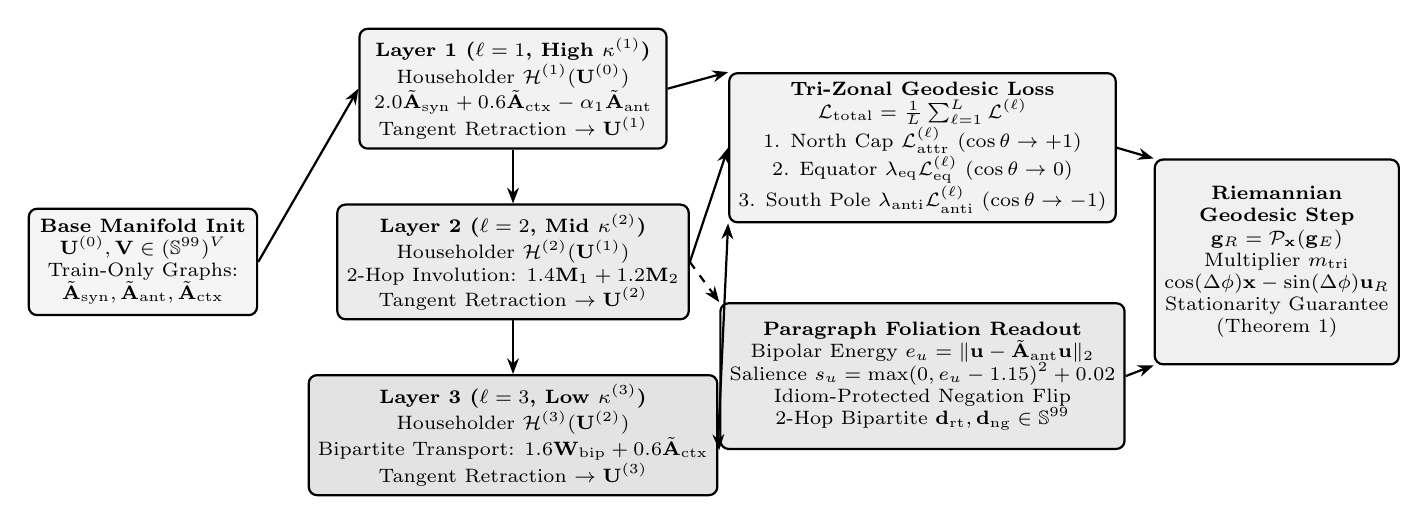
\begin{tikzpicture}[every node/.style={font=\scriptsize, text=black}]
% Inputs on Left
\node[draw=black, thick, fill=gray!8, rounded corners=3pt, minimum width=2.9cm, minimum height=1.35cm, align=center] (inputs) at (-7.1, 0) {\textbf{Base Manifold Init}\\$\mathbf{U}^{(0)}, \mathbf{V} \in (\mathbb{S}^{99})^V$\\Train-Only Graphs:\\$\tilde{\mathbf{A}}_{\text{syn}}, \tilde{\mathbf{A}}_{\text{ant}}, \tilde{\mathbf{A}}_{\text{ctx}}$};

% Layer 1
\node[draw=black, thick, fill=gray!10, rounded corners=3pt, minimum width=3.9cm, minimum height=1.35cm, align=center] (layer1) at (-2.4, 2.2) {\textbf{Layer 1 ($\ell=1$, High $\kappa^{(1)}$)}\\Householder $\mathcal{H}^{(1)}(\mathbf{U}^{(0)})$\\$2.0\tilde{\mathbf{A}}_{\text{syn}} + 0.6\tilde{\mathbf{A}}_{\text{ctx}} - \alpha_1\tilde{\mathbf{A}}_{\text{ant}}$\\Tangent Retraction $\to \mathbf{U}^{(1)}$};

% Layer 2
\node[draw=black, thick, fill=gray!16, rounded corners=3pt, minimum width=3.9cm, minimum height=1.35cm, align=center] (layer2) at (-2.4, 0.0) {\textbf{Layer 2 ($\ell=2$, Mid $\kappa^{(2)}$)}\\Householder $\mathcal{H}^{(2)}(\mathbf{U}^{(1)})$\\2-Hop Involution: $1.4\mathbf{M}_1 + 1.2\mathbf{M}_2$\\Tangent Retraction $\to \mathbf{U}^{(2)}$};

% Layer 3
\node[draw=black, thick, fill=gray!22, rounded corners=3pt, minimum width=3.9cm, minimum height=1.35cm, align=center] (layer3) at (-2.4, -2.2) {\textbf{Layer 3 ($\ell=3$, Low $\kappa^{(3)}$)}\\Householder $\mathcal{H}^{(3)}(\mathbf{U}^{(2)})$\\Bipartite Transport: $1.6\mathbf{W}_{\text{bip}} + 0.6\tilde{\mathbf{A}}_{\text{ctx}}$\\Tangent Retraction $\to \mathbf{U}^{(3)}$};

% Tri-Zonal Objective Box
\node[draw=black, thick, fill=gray!10, rounded corners=3pt, minimum width=4.0cm, minimum height=1.85cm, align=center] (loss) at (2.8, 1.45) {\textbf{Tri-Zonal Geodesic Loss}\\$\mathcal{L}_{\text{total}} = \frac{1}{L}\sum_{\ell=1}^L \mathcal{L}^{(\ell)}$\\1. North Cap $\mathcal{L}_{\text{attr}}^{(\ell)}$ ($\cos\theta \to +1$)\\2. Equator $\lambda_{\text{eq}}\mathcal{L}_{\text{eq}}^{(\ell)}$ ($\cos\theta \to 0$)\\3. South Pole $\lambda_{\text{anti}}\mathcal{L}_{\text{anti}}^{(\ell)}$ ($\cos\theta \to -1$)};

% Document Transport & Negation Box
\node[draw=black, thick, fill=gray!18, rounded corners=3pt, minimum width=4.0cm, minimum height=1.85cm, align=center] (doc) at (2.8, -1.45) {\textbf{Paragraph Foliation Readout}\\Bipolar Energy $e_u = \|\mathbf{u} - \tilde{\mathbf{A}}_{\text{ant}}\mathbf{u}\|_2$\\Salience $s_u = \max(0, e_u - 1.15)^2 + 0.02$\\Idiom-Protected Negation Flip\\2-Hop Bipartite $\mathbf{d}_{\text{rt}}, \mathbf{d}_{\text{ng}} \in \mathbb{S}^{99}$};

% Riemannian Optimizer Box
\node[draw=black, thick, fill=gray!12, rounded corners=3pt, minimum width=3.1cm, minimum height=2.6cm, align=center] (opt) at (7.3, 0.0) {\textbf{Riemannian}\\ \textbf{Geodesic Step}\\$\mathbf{g}_R = \mathcal{P}_{\mathbf{x}}(\mathbf{g}_E)$\\Multiplier $m_{\text{tri}}$\\$\cos(\Delta\phi)\mathbf{x} - \sin(\Delta\phi)\mathbf{u}_R$\\Stationarity Guarantee\\(Theorem 1)};

% Connections
\draw[-{Stealth[length=2mm]}, thick, black] (inputs.east) -- (layer1.west);
\draw[-{Stealth[length=2mm]}, thick, black] (layer1.south) -- (layer2.north);
\draw[-{Stealth[length=2mm]}, thick, black] (layer2.south) -- (layer3.north);

\draw[-{Stealth[length=2mm]}, thick, black] (layer1.east) -- (loss.north west);
\draw[-{Stealth[length=2mm]}, thick, black] (layer2.east) -- (loss.west);
\draw[-{Stealth[length=2mm]}, thick, black] (layer3.east) -- (loss.south west);

\draw[-{Stealth[length=2mm]}, thick, black, dashed] (layer2.east) -- (doc.north west);
\draw[-{Stealth[length=2mm]}, thick, black, dashed] (layer3.east) -- (doc.south west);

\draw[-{Stealth[length=2mm]}, thick, black] (loss.east) -- (opt.north west);
\draw[-{Stealth[length=2mm]}, thick, black] (doc.east) -- (opt.south west);
\end{tikzpicture}%
}
\caption{End-to-end architecture and optimization workflow of POLARIS. Base word embeddings on $\mathbb{S}^{99}$ pass through three concentric Householder-reflected spherical layers with decreasing directional concentration ($\kappa^{(1)} > \kappa^{(2)} > \kappa^{(3)}$). Layer 2 feeds lexical polarity representations and bipolar salience to sentiment document readout ($\mathbf{d}_{\text{rt}}$), whereas Layer 3 provides topic-transported representations for multi-class document clustering and classification ($\mathbf{d}_{\text{ng}}$).}
\label{fig:polaris_workflow}
\end{figure*}

\subsection{Overall Framework}
Fig.~\ref{fig:polaris_workflow} depicts the end-to-end architecture of POLARIS. Rather than forcing a single embedding matrix to satisfy conflicting local polarity and global topical objectives, POLARIS transforms base spherical embeddings $\mathbf{U}^{(0)} \in (\mathbb{S}^{p-1})^V$ through $L = 3$ concentric spherical layers $\{\mathbf{U}^{(1)}, \mathbf{U}^{(2)}, \mathbf{U}^{(3)}\}$. At each layer $\ell \in \{1, \dots, L\}$, embeddings first undergo an isometric orthogonal rotation and reflection via a chain of $K_h = 4$ Householder reflections $\mathcal{H}^{(\ell)}$. Next, layer-specific graph propagation computes an ambient drift vector $\mathbf{Z}^{(\ell)}$ that transitions from 1-hop signed lexical attraction/repulsion ($\ell = 1$), to 2-hop signed geodesic involution ($\ell = 2$), to bipartite word-document-word topic transport ($\ell = 3$). Each ambient drift is projected onto the local tangent space via (\ref{eq:tangent_proj}), scaled by a step size coupled to the learned concentration parameter $\kappa^{(\ell)}$, and retracted onto $\mathbb{S}^{p-1}$ via (\ref{eq:retraction}). All layers are jointly supervised by the Tri-Zonal Geodesic Loss and updated using Riemannian tangential geodesic steps.

\subsection{Main Architectural Components}

\subsubsection{Isometric Orthogonal Householder Reflection Chains}
One may ask why we connect consecutive spherical layers using chains of Householder reflections rather than standard dense linear transformations $\mathbf{W}^{(\ell)} \in \mathbb{R}^{p \times p}$ followed by $\ell_2$ normalization. Why not simply use an unconstrained matrix multiplication? The answer lies in both metric preservation and algorithmic complexity. An unconstrained matrix $\mathbf{W}^{(\ell)}$ alters vector norms along its singular directions, distorting geodesic angles prior to retraction, and requires $p^2 = 10,000$ parameters and $\mathcal{O}(Vp^2)$ floating-point operations per layer. Moreover, maintaining orthogonality on the Stiefel manifold via matrix exponential or Cayley retraction requires expensive $\mathcal{O}(p^3)$ matrix inversions \cite{mhammedi2017efficient}.

Instead, we parameterize the inter-layer orthogonal transition $\mathcal{H}^{(\ell)}: (\mathbb{S}^{p-1})^V \to (\mathbb{S}^{p-1})^V$ as a composition of $K_h = 4$ Householder reflections:
\begin{equation}
\mathcal{H}^{(\ell)}(\mathbf{X}) = \mathbf{X} \prod_{k=1}^{K_h} \mathbf{H}\!\left(\mathbf{q}^{(\ell,k)}\right), \quad \mathbf{H}(\mathbf{q}) = \mathbf{I}_p - 2\mathbf{q}\mathbf{q}^\top,
\label{eq:householder}
\end{equation}
where each normal vector $\mathbf{q}^{(\ell,k)} \in \mathbb{S}^{p-1}$ is a learnable unit vector on the hypersphere. Every individual reflection $\mathbf{H}(\mathbf{q})$ is symmetric ($\mathbf{H}^\top = \mathbf{H}$) and orthogonal ($\mathbf{H}^\top \mathbf{H} = \mathbf{I}_p - 4\mathbf{q}\mathbf{q}^\top + 4\mathbf{q}(\mathbf{q}^\top\mathbf{q})\mathbf{q}^\top = \mathbf{I}_p$), ensuring that $\|\mathbf{x}^\top \mathbf{H}(\mathbf{q})\|_2 = \|\mathbf{x}\|_2 = 1$ holds identically without post-hoc normalization. Furthermore, we never instantiate the $p \times p$ matrix $\mathbf{H}(\mathbf{q})$; instead, each reflection is evaluated sequentially via vector-vector inner products:
\begin{equation}
\mathbf{x}_{k} = \mathbf{x}_{k-1} - 2\left(\mathbf{x}_{k-1}^\top \mathbf{q}^{(\ell,k)}\right)\mathbf{q}^{(\ell,k)},
\label{eq:householder_fast}
\end{equation}
which reduces time complexity from $\mathcal{O}(Vp^2)$ to $\mathcal{O}(K_h V p) = \mathcal{O}(Vp)$ and requires only $L K_h p = 3 \times 4 \times 100 = 1,200$ parameters across the entire 3-layer network.

\subsubsection{Self-Calibrating Monotonic Concentration Cascade}
On the unit hypersphere, the directional concentration parameter $\kappa > 0$ of the vMF likelihood $\exp(\kappa \mathbf{u}^\top \mathbf{v})$ controls the angular resolution of neighborhood boundaries. Why not fix $\kappa = 1$ across all layers? If $\kappa$ is fixed to unity, the log-sigmoid inner-product loss $\log \sigma(\kappa \cos\theta)$ varies only between $\log\sigma(-1) = -1.313$ and $\log\sigma(+1) = -0.313$, generating weak tangential gradients that fail to compress multi-class topical clusters. Conversely, if a single high $\kappa$ is forced on all layers, tight local lexical clusters fracture broad document topics.

To resolve this multi-scale tension, we design a self-calibrating monotonic concentration cascade that enforces strict ordering $\kappa^{(1)} > \kappa^{(2)} > \dots > \kappa^{(L)} > \kappa_{\text{base}}$ throughout training. Given base concentration $\kappa_{\text{base}} = 2.0$ and learnable unconstrained scalars $\tilde{\delta}_1, \dots, \tilde{\delta}_L \in \mathbb{R}$ (initialized to $[0.95, 0.75, 0.60]$ for $L=3$), we define positive increments $\Delta\kappa_\ell = \text{softplus}(\tilde{\delta}_\ell) = \log(1 + \exp(\tilde{\delta}_\ell)) > 0$ and accumulate them in reverse layer order:
\begin{equation}
\kappa^{(\ell)} = \kappa_{\text{base}} + \sum_{j=\ell}^{L} \log\!\left(1 + \exp(\tilde{\delta}_j)\right), \quad \ell \in \{1, \dots, L\}.
\label{eq:kappa_cascade}
\end{equation}
Because $\log(1 + \exp(\tilde{\delta}_j)) > 0$ for all finite $\tilde{\delta}_j$, (\ref{eq:kappa_cascade}) mathematically guarantees $\kappa^{(1)} > \kappa^{(2)} > \kappa^{(3)} > 2.0$ without constrained projection steps.

\subsubsection{Concentric Layer-Wise Foliation and Signed Geodesic Involution}
Let $\tilde{\mathbf{U}}^{(\ell)} = \mathcal{H}^{(\ell)}(\mathbf{U}^{(\ell-1)}) \in (\mathbb{S}^{p-1})^V$ denote the Householder-rotated embeddings entering layer $\ell$, and let $\alpha_\ell = 1.35\,\sigma(\hat{\alpha}_\ell) \in (0, 1.35)$ denote a learnable antipodal repulsion gate. Each concentric layer computes a specialized ambient drift $\mathbf{Z}^{(\ell)} \in \mathbb{R}^{V \times p}$ before projecting onto the tangent bundle:

\paragraph{Layer 1 (1-Hop Signed Lexical and Contextual Drift)}
In the first layer ($\ell = 1$), operating at the highest concentration $\kappa^{(1)}$, each word aggregates direct 1-hop attraction from WordNet synonyms and non-antonymous corpus co-occurrences while experiencing direct antipodal repulsion from 1-hop antonyms:
\begin{equation}
\mathbf{Z}^{(1)} = 2.0\tilde{\mathbf{A}}_{\text{syn}}\tilde{\mathbf{U}}^{(1)} + 0.6\tilde{\mathbf{A}}_{\text{ctx}}\tilde{\mathbf{U}}^{(1)} - \alpha_1\tilde{\mathbf{A}}_{\text{ant}}\tilde{\mathbf{U}}^{(1)}.
\label{eq:layer1_drift}
\end{equation}
Subtracting $\alpha_1\tilde{\mathbf{A}}_{\text{ant}}\tilde{\mathbf{U}}^{(1)}$ injects a tangent displacement directed toward $-\tilde{\mathbf{u}}_{v^-}^{(1)}$, initiating the migration of direct antonyms toward the South Pole.

\paragraph{Layer 2 (2-Hop Signed Geodesic Involution)}
Why is 1-hop repulsion insufficient for complete lexical polarity separation? Because lexical graphs are sparse: many semantically opposite word pairs are separated by two hops (for example, an antonym of a synonym, or a synonym of an antonym), and two words that share a common antonym are themselves synonymous. In Layer 2 ($\ell = 2$), we define the 1-hop and 2-hop signed involution operators:
\begin{equation}
\mathbf{M}_1 = \left(\tilde{\mathbf{A}}_{\text{syn}} - \tilde{\mathbf{A}}_{\text{ant}}\right)\tilde{\mathbf{U}}^{(2)},
\label{eq:inv1}
\end{equation}
\begin{equation}
\begin{aligned}
\mathbf{M}_2 &= \left(\tilde{\mathbf{A}}_{\text{syn}} - \tilde{\mathbf{A}}_{\text{ant}}\right)\mathbf{M}_1 \\
&= \left(\tilde{\mathbf{A}}_{\text{syn}}^2 - \tilde{\mathbf{A}}_{\text{syn}}\tilde{\mathbf{A}}_{\text{ant}} - \tilde{\mathbf{A}}_{\text{ant}}\tilde{\mathbf{A}}_{\text{syn}} + \tilde{\mathbf{A}}_{\text{ant}}^2\right)\tilde{\mathbf{U}}^{(2)}.
\end{aligned}
\label{eq:inv2}
\end{equation}
Expanding $\mathbf{M}_2$ reveals its algebraic symmetry: two consecutive synonym hops ($+\tilde{\mathbf{A}}_{\text{syn}}^2$) and two consecutive antonym hops ($+\tilde{\mathbf{A}}_{\text{ant}}^2$) carry a positive sign, pulling antonyms-of-antonyms back toward the North Pole ($\cos\theta \to +1$), whereas mixed synonym-antonym paths ($-\tilde{\mathbf{A}}_{\text{syn}}\tilde{\mathbf{A}}_{\text{ant}} - \tilde{\mathbf{A}}_{\text{ant}}\tilde{\mathbf{A}}_{\text{syn}}$) carry a negative sign, pushing 2-hop opposites toward the South Pole ($\cos\theta \to -1$). The Layer 2 ambient drift combines both involution orders with local context:
\begin{equation}
\mathbf{Z}^{(2)} = 1.4\mathbf{M}_1 + 1.2\mathbf{M}_2 + 0.4\tilde{\mathbf{A}}_{\text{ctx}}\tilde{\mathbf{U}}^{(2)}.
\label{eq:layer2_drift}
\end{equation}

\paragraph{Layer 3 (Bipartite Word-Document-Word Spherical Transport)}
In Layer 3 ($\ell = 3$), operating at lower concentration $\kappa^{(3)}$ to capture broader semantic neighborhoods, we couple the lexical graph with global document topic structure via two-step bipartite transport over the normalized document-word TF-IDF matrix $\mathbf{M}_{\text{ng}} \in \mathbb{R}^{N_{\text{ng}} \times V}$:
\begin{equation}
\mathbf{D}_{\text{topic}} = \mathcal{R}_{\mathbb{S}}\!\left(\mathbf{M}_{\text{ng}}\tilde{\mathbf{U}}^{(3)}\right), \quad \mathbf{W}_{\text{bip}} = \mathcal{R}_{\mathbb{S}}\!\left(\mathbf{M}_{\text{ng}}^\top \mathbf{D}_{\text{topic}}\right),
\label{eq:bip_transport}
\end{equation}
\begin{equation}
\begin{aligned}
\mathbf{Z}^{(3)} &= 1.6\mathbf{W}_{\text{bip}} + 0.6\tilde{\mathbf{A}}_{\text{ctx}}\tilde{\mathbf{U}}^{(3)} \\
&\quad + 0.6\left(\tilde{\mathbf{A}}_{\text{syn}}\tilde{\mathbf{U}}^{(3)} - \alpha_3\tilde{\mathbf{A}}_{\text{ant}}\tilde{\mathbf{U}}^{(3)}\right).
\end{aligned}
\label{eq:layer3_drift}
\end{equation}
Here, $\mathbf{D}_{\text{topic}} \in (\mathbb{S}^{p-1})^{N_{\text{ng}}}$ aggregates word vectors into spherical document centroids, and $\mathbf{W}_{\text{bip}} \in (\mathbb{S}^{p-1})^V$ transports those document centroids back to the constituent words, aligning words that share global topical documents even when they do not directly co-occur within a 5-word sliding window. (For depth sensitivity experiments with $\ell > 3$, higher layers apply regularized contextual smoothing $\mathbf{Z}^{(\ell)} = (1 + 0.5(\ell - 3))^{-1}\tilde{\mathbf{A}}_{\text{ctx}}\tilde{\mathbf{U}}^{(\ell)} + 0.2(\ell - 3)\boldsymbol{\epsilon}$ with $\boldsymbol{\epsilon} \sim \mathcal{N}(\mathbf{0}, \mathbf{I}_p)$.)

Finally, across every layer $\ell \in \{1, \dots, L\}$, the ambient drift $\mathbf{Z}^{(\ell)}$ is projected onto the tangent space of $\tilde{\mathbf{U}}^{(\ell)}$ and retracted onto $\mathbb{S}^{p-1}$:
\begin{equation}
\mathbf{u}_i^{(\ell)} = \mathcal{R}_{\tilde{\mathbf{u}}_i^{(\ell)}}\!\left(\gamma_\ell \, \mathcal{P}_{\tilde{\mathbf{u}}_i^{(\ell)}}\!\left(\mathbf{z}_i^{(\ell)}\right)\right), \quad \gamma_\ell = 0.65\,\sigma(\hat{\gamma}_\ell)\frac{\kappa^{(\ell)}}{2.0},
\label{eq:layer_update}
\end{equation}
where $\hat{\gamma}_\ell \in \mathbb{R}$ is a learnable step parameter.

\subsubsection{Intrinsic Bipolar Energy and Polarity-Gated Negation Reflection}
When constructing document embeddings on $\mathbb{S}^{p-1}$, a major shortcoming of standard TF-IDF aggregation is that neutral topical words drown out sentiment-bearing words, and negated expressions fail to invert direction. Because POLARIS places antonyms in opposing hemispheres ($\mathbf{v}^- \approx -\mathbf{u}$), we can quantify the intrinsic polarity salience of any word $u \in \mathcal{V}$ directly from the geometry of Layer 2 embeddings $\mathbf{U}^{(2)}$ without external sentiment lexicons. We define the Intrinsic Spherical Bipolar Energy $e_u$ and salience weight $s_u$ as:
\begin{equation}
\begin{aligned}
e_u &= \left\|\mathbf{u}_u^{(2)} - \left(\tilde{\mathbf{A}}_{\text{ant}}\mathbf{U}^{(2)}\right)_u\right\|_2, \\
s_u &= \max\!\left(0, \, e_u - 1.15\right)^2 + 0.02.
\end{aligned}
\label{eq:bipolar_energy}
\end{equation}
Why does $e_u$ isolate polarity-bearing words? For a neutral word $u$ that has no antonyms in $\tilde{\mathbf{A}}_{\text{ant}}$, $(\tilde{\mathbf{A}}_{\text{ant}}\mathbf{U}^{(2)})_u = \mathbf{0}$, so $e_u = \|\mathbf{u}_u^{(2)}\|_2 = 1.0 < 1.15$, assigning $u$ a baseline weight of $s_u = 0.02$. Conversely, for a polarized word $u$ whose antonyms lie near the opposite pole ($\tilde{\mathbf{A}}_{\text{ant}}\mathbf{u}_u^{(2)} \approx -\mathbf{u}_u^{(2)}$), the chordal distance approaches $e_u \approx \|\mathbf{u}_u^{(2)} - (-\mathbf{u}_u^{(2)})\|_2 \to 2.0$, boosting its salience weight up to $s_u \approx (2.0 - 1.15)^2 + 0.02 = 0.7425$.

In addition, during tokenization of document $d$, whenever a negation cue (e.g., \textit{not, never, no, without, fails, cannot}) is encountered, we activate a 3-token negation scope countdown ($\tau_{\text{neg}} = 3$) over subsequent content words while protecting positive idioms containing negation tokens (specifically \textit{"not only"}, \textit{"not just"}, \textit{"without a doubt"}, \textit{"no doubt"}, \textit{"never fails"}, \textit{"cannot wait"}, \textit{"nothing short of"}, and \textit{"no wonder"}). For each token occurrence $w$ in document $d$, its effective polarity sign $\sigma_{d,w} \in \{-1, +1\}$ is gated by membership in the training polarity node set $\mathcal{V}_{\text{pol}}$:
\begin{equation}
\sigma_{d,w} = \begin{cases}
-1, & \text{if } w \in \mathcal{V}_{\text{pol}} \text{ and } \tau_{\text{neg}} > 0, \\
+1, & \text{otherwise.}
\end{cases}
\label{eq:negation_gate}
\end{equation}
Multiplying $\mathbf{u}_w^{(2)}$ by $\sigma_{d,w} = -1$ reflects the word vector across the origin to its antipode $-\mathbf{u}_w^{(2)} \in \mathbb{S}^{p-1}$, so that \textit{"not good"} maps directly into the Southern Hemisphere region occupied by \textit{"bad"} and \textit{"stale"}. Both topical document embeddings $\mathbf{d}_{\text{ng}}$ (from Layer 3 using unsigned matrix $\mathbf{M}_{\text{ng}}$) and sentiment document embeddings $\mathbf{d}_{\text{rt}}$ (from Layer 2 using signed matrix $\mathbf{M}_{\text{rt}}^{(s)}$ and bipolar salience $s_u$) undergo 2-hop bipartite spherical refinement:
\begin{equation}
\begin{aligned}
\mathbf{d}_{\text{rt}}^{(1)} &= \mathcal{R}_{\mathbb{S}}\!\left(\mathbf{M}_{\text{rt}}^{(s)} \operatorname{diag}(\mathbf{s})\mathbf{U}^{(2)}\right), \\
\mathbf{d}_{\text{rt}} &= \mathcal{R}_{\mathbb{S}}\!\left(\mathbf{M}_{\text{rt}}^{(s)} \, \mathcal{R}_{\mathbb{S}}\!\left(\mathbf{M}_{\text{rt}}^{(s)\top}\mathbf{d}_{\text{rt}}^{(1)}\right)\right),
\end{aligned}
\label{eq:doc_rt}
\end{equation}
\begin{equation}
\begin{aligned}
\mathbf{d}_{\text{ng}}^{(1)} &= \mathcal{R}_{\mathbb{S}}\!\left(\mathbf{M}_{\text{ng}}\mathbf{U}^{(3)}\right), \\
\mathbf{d}_{\text{ng}} &= \mathcal{R}_{\mathbb{S}}\!\left(\mathbf{M}_{\text{ng}} \, \mathcal{R}_{\mathbb{S}}\!\left(\mathbf{M}_{\text{ng}}^\top\mathbf{d}_{\text{ng}}^{(1)}\right)\right).
\end{aligned}
\label{eq:doc_ng}
\end{equation}

\subsection{Tri-Zonal Geodesic Loss Functions}
To enforce the three geometric zones on $\mathbb{S}^{p-1}$ across all $L$ layers, we minimize the multi-layer Tri-Zonal Geodesic Loss:
\begin{equation}
\mathcal{L}_{\text{total}}(\boldsymbol{\Theta}) = \frac{1}{L}\sum_{\ell=1}^{L} \left( \mathcal{L}_{\text{attr}}^{(\ell)} + \lambda_{\text{anti}}\mathcal{L}_{\text{anti}}^{(\ell)} + \lambda_{\text{eq}}\mathcal{L}_{\text{eq}}^{(\ell)} \right),
\label{eq:total_loss}
\end{equation}
where $\lambda_{\text{anti}} = 1.5$ and $\lambda_{\text{eq}} = 0.25$ balance the three zones. Each term in (\ref{eq:total_loss}) serves a distinct geometric function:

\subsubsection{North Polar Cap Attraction Zone ($\mathcal{L}_{\text{attr}}^{(\ell)}$)}
The attraction loss pulls co-occurring words, synonyms, and document-word pairs toward $\cos\theta \to +1.0$:
\begin{equation}
\mathcal{L}_{\text{attr}}^{(\ell)} = \mathcal{L}_{\text{cooc}}^{(\ell)} + 1.6\mathcal{L}_{\text{syn}}^{(\ell)} + 0.5\left(\mathcal{L}_{\text{doc,rt}}^{(\ell)} + \mathcal{L}_{\text{doc,ng}}^{(\ell)}\right),
\label{eq:loss_attr}
\end{equation}
where the concentration-scaled directional log-sigmoid losses and hybrid hinge-quadratic synonym attraction loss are defined as:
\begin{equation}
\begin{aligned}
\mathcal{L}_{\text{cooc}}^{(\ell)} = -\mathbb{E}_{(u,v), n}\Big[ w_{uv}\Big(&\log\sigma\!\left(\kappa^{(\ell)}\mathbf{u}_u^{(\ell)\top}\mathbf{v}_v\right) \\
&+ \log\sigma\!\left(-\kappa^{(\ell)}\mathbf{u}_n^{(\ell)\top}\mathbf{v}_v\right)\Big) \Big],
\end{aligned}
\label{eq:loss_cooc}
\end{equation}
\begin{equation}
\begin{aligned}
\mathcal{L}_{\text{syn}}^{(\ell)} = \mathbb{E}_{(u,v^+)\sim\mathcal{E}_{\text{syn}}}\Big[ &\max\!\left(0, \, 0.92 - \mathbf{u}_u^{(\ell)\top}\mathbf{u}_{v^+}^{(\ell)}\right) \\
&+ 0.35\left(1.0 - \mathbf{u}_u^{(\ell)\top}\mathbf{u}_{v^+}^{(\ell)}\right)^2 \Big],
\end{aligned}
\label{eq:loss_syn}
\end{equation}
\begin{equation}
\begin{aligned}
\mathcal{L}_{\text{doc,rt}}^{(\ell)} = -\mathbb{E}_{(d,w), n}\Big[ &\log\sigma\!\left(\kappa^{(\ell)}\sigma_{d,w}\mathbf{u}_w^{(\ell)\top}\mathbf{d}_d^{\text{rt}}\right) \\
&+ \log\sigma\!\left(-\kappa^{(\ell)}\mathbf{u}_n^{(\ell)\top}\mathbf{d}_d^{\text{rt}}\right) \Big].
\end{aligned}
\label{eq:loss_doc}
\end{equation}
The topical document loss $\mathcal{L}_{\text{doc,ng}}^{(\ell)}$ is identical to (\ref{eq:loss_doc}) with unsigned indicator $\sigma_{d,w} = +1$ and document parameter $\mathbf{d}_d^{\text{ng}}$. Combining a linear hinge margin ($m_{\text{syn}} = 0.92$) with a smooth quadratic pull ($0.35(1 - \cos\theta)^2$) in (\ref{eq:loss_syn}) provides constant gradient magnitude when synonyms are far apart while maintaining smooth second-order curvature near the North Pole ($\cos\theta \to +1$).

\subsubsection{South Antipodal Pole Repulsion Zone ($\mathcal{L}_{\text{anti}}^{(\ell)}$)}
To push antonym pairs $(u, v^-) \in \mathcal{E}_{\text{ant}}$ into the Southern Hemisphere toward the antipodal target ($\mathbf{u}_{v^-}^{(\ell)} \to -\mathbf{u}_u^{(\ell)}$, or $\cos\theta \to -1.0$), we formulate the hybrid hinge-quadratic antipodal loss:
\begin{equation}
\begin{aligned}
\mathcal{L}_{\text{anti}}^{(\ell)} = \mathbb{E}_{(u,v^-)\sim\mathcal{E}_{\text{ant}}}\Big[ &\max\!\left(0, \, 0.88 + \mathbf{u}_u^{(\ell)\top}\mathbf{u}_{v^-}^{(\ell)}\right) \\
&+ 0.45\left(1.0 + \mathbf{u}_u^{(\ell)\top}\mathbf{u}_{v^-}^{(\ell)}\right)^2 \Big].
\end{aligned}
\label{eq:loss_anti}
\end{equation}
Why combine the linear hinge margin ($\cos\theta \le -0.88$, or $\theta \ge 151.6^\circ$) with the smooth quadratic potential $0.45(1 + \cos\theta)^2$? A pure hinge loss (such as $\cos\theta \le -0.25$ in Attract-Repel \cite{mrksic2017semantic}) has zero gradient once the threshold is crossed, leaving antonyms nearly orthogonal. Conversely, in (\ref{eq:loss_anti}), the linear hinge provides a strong constant-slope repulsive force whenever $\cos\theta > -0.88$, while the quadratic potential $(1 + \mathbf{u}_u^\top \mathbf{u}_{v^-})^2 = \frac{1}{4}\|\mathbf{u}_u + \mathbf{u}_{v^-}\|_2^4$ continues exerting a smooth, diminishing tangential pull toward $\cos\theta = -1.0$ even after the hinge deactivates at $-0.88$. In practice, because words simultaneously experience distributional attraction $\mathcal{L}_{\text{cooc}}^{(\ell)}$ from shared context words and participate in multi-antonym cliques (where a single vector $\mathbf{u}_u$ cannot simultaneously lie at $-1.0$ cosine to multiple distinct antonym vectors), the multi-objective equilibrium settles at a strong negative mean cosine of $\cos\theta_{\text{ant}} = -0.764 \pm 0.000$ ($\text{AAS} = 0.6108$), while isolated high-salience pairs reach $-0.909$ to $-0.977$ (Table~\ref{tab:exp7_qualitative}).

\subsubsection{Equatorial Orthogonality Zone ($\mathcal{L}_{\text{eq}}^{(\ell)}$)}
If a spherical model only pushes synonyms toward $+1$ and antonyms toward $-1$, unrelated words can drift into either polar cap or form dense hubs that degrade nearest-neighbor retrieval. We regularize unrelated random pairs $(u, n)$ toward the equatorial belt ($\cos\theta_{un} \to 0$, or $\theta_{un} \to \pi/2$):
\begin{equation}
\begin{aligned}
\mathcal{L}_{\text{eq}}^{(\ell)} = \mathbb{E}_{(u,n)}\Big[ &\max\!\left(0, \, \left|\mathbf{u}_u^{(\ell)\top}\mathbf{u}_n^{(\ell)}\right| - 0.08\right)^2 \\
&+ 0.25\left(\mathbf{u}_u^{(\ell)\top}\mathbf{u}_n^{(\ell)}\right)^2 \Big].
\end{aligned}
\label{eq:loss_eq}
\end{equation}
Allowing a dead-zone band of $|\cos\theta_{un}| \le 0.08$ prevents over-constraining words that happen to share macro-level topics while penalizing spurious high-cosine hubness.

\begin{algorithm}[!t]
\caption{POLARIS Training and Foliation Procedure}
\label{alg:polaris}
\footnotesize
\begin{algorithmic}[1]
\Require Vocabulary $\mathcal{V}$ ($V=8,000$), Co-occurrence pairs $\mathcal{E}_{\text{cooc}}$, Train-only WordNet graphs $\tilde{\mathbf{A}}_{\text{syn}}, \tilde{\mathbf{A}}_{\text{ant}}, \tilde{\mathbf{A}}_{\text{ctx}}$, Document matrices $\mathbf{M}_{\text{rt}}^{(s)}, \mathbf{M}_{\text{ng}}$, Layers $L=3$, Reflections $K_h=4$, Dimension $p=100$, Epochs $E=14$.
\Ensure Multi-layer word embeddings $\{\mathbf{U}^{(\ell)}\}_{\ell=1}^L$ and document embeddings $\mathbf{d}_{\text{rt}}, \mathbf{d}_{\text{ng}} \in \mathbb{S}^{p-1}$.
\State Initialize $\mathbf{U}^{(0)} \sim \mathcal{U}(\mathbb{S}^{p-1})^V$, $\mathbf{V} \leftarrow \mathbf{U}^{(0)}$, $\mathbf{q}^{(\ell,k)} \sim \mathcal{U}(\mathbb{S}^{p-1})$.
\State Initialize $\mathbf{d}_{\text{rt}} \leftarrow \mathcal{R}_{\mathbb{S}}(\mathbf{M}_{\text{rt}}^{(s)}\mathbf{U}^{(0)})$, $\mathbf{d}_{\text{ng}} \leftarrow \mathcal{R}_{\mathbb{S}}(\mathbf{M}_{\text{ng}}\mathbf{U}^{(0)})$.
\For{epoch $e = 1$ \textbf{to} $E$}
    \State Set geodesic learning rate $\eta_e = 0.045 \left(1 - 0.5\frac{e-1}{E-1}\right)$.
    \For{each mini-batch $\mathcal{B} \subset \mathcal{E}_{\text{cooc}}$ of size $|\mathcal{B}| = 24,000$}
        \State Compute cascade $\kappa^{(1)} > \kappa^{(2)} > \kappa^{(3)} > 2.0$ via (\ref{eq:kappa_cascade}).
        \For{layer $\ell = 1$ \textbf{to} $L$}
            \State Apply reflections $\tilde{\mathbf{U}}^{(\ell)} = \mathcal{H}^{(\ell)}(\mathbf{U}^{(\ell-1)})$ via (\ref{eq:householder_fast}).
            \State Compute drift $\mathbf{Z}^{(\ell)}$ via (\ref{eq:layer1_drift}), (\ref{eq:layer2_drift}), or (\ref{eq:layer3_drift}).
            \State Retract $\mathbf{U}^{(\ell)} = \mathcal{R}_{\tilde{\mathbf{U}}^{(\ell)}}(\gamma_\ell \mathcal{P}_{\tilde{\mathbf{U}}^{(\ell)}}(\mathbf{Z}^{(\ell)}))$ via (\ref{eq:layer_update}).
            \State Evaluate $\mathcal{L}_{\text{attr}}^{(\ell)}, \mathcal{L}_{\text{anti}}^{(\ell)}, \mathcal{L}_{\text{eq}}^{(\ell)}$ via (\ref{eq:loss_attr})--(\ref{eq:loss_eq}).
        \EndFor
        \State Backpropagate $\mathcal{L}_{\text{total}} = \frac{1}{L}\sum_{\ell=1}^L (\mathcal{L}_{\text{attr}}^{(\ell)} + 1.5\mathcal{L}_{\text{anti}}^{(\ell)} + 0.25\mathcal{L}_{\text{eq}}^{(\ell)})$.
        \State Update 12 scalar gates $\{\hat{\gamma}_\ell, \hat{\alpha}_\ell, \tilde{\delta}_\ell, w_\ell\}$ via Adam ($\text{lr}=0.025$).
        \For{each $\mathbf{x} \in \{\mathbf{U}^{(0)}, \mathbf{V}, \mathbf{q}^{(\ell,k)}, \mathbf{d}_{\text{rt}}, \mathbf{d}_{\text{ng}}\}$ with scale $c_{\mathbf{x}}$}
            \State Project gradient: $\mathbf{g}_{\text{riem}} = \mathbf{g}_{\text{euc}} - (\mathbf{x}^\top\mathbf{g}_{\text{euc}})\mathbf{x}$.
            \State Set $m_{\text{tri}} = \operatorname{clip}(1.15 + 0.85 (\mathbf{x}^\top\mathbf{g}_{\text{euc}})/\|\mathbf{g}_{\text{euc}}\|_2, 0.2, 2.0)$.
            \State Set $\Delta\phi = \min(0.35, c_{\mathbf{x}}\eta_e m_{\text{tri}})$ and $\mathbf{u}_R = \mathbf{g}_{\text{riem}}/\|\mathbf{g}_{\text{riem}}\|_2$.
            \State Update $\mathbf{x} \leftarrow \mathcal{R}_{\mathbb{S}}(\cos(\Delta\phi)\mathbf{x} - \sin(\Delta\phi)\mathbf{u}_R)$.
        \EndFor
    \EndFor
\EndFor
\State Compute salience $s_u$ via (\ref{eq:bipolar_energy}) and $\mathbf{d}_{\text{rt}}, \mathbf{d}_{\text{ng}}$ via (\ref{eq:doc_rt})--(\ref{eq:doc_ng}).
\end{algorithmic}
\end{algorithm}

\subsection{Riemannian Optimization, Convergence Analysis, and Complexity}
Algorithm~\ref{alg:polaris} details the complete training procedure of POLARIS. Optimization separates into two parameter groups: (i) the $12$ unconstrained scalar gate and concentration parameters $\boldsymbol{\psi} = \{\hat{\gamma}_\ell, \hat{\alpha}_\ell, \tilde{\delta}_\ell, w_\ell\}_{\ell=1}^3 \in \mathbb{R}^{12}$, which are updated via Adam ($\text{lr}=0.025$), and (ii) the $M = 2V + LK_h + N_{\text{rt}} + N_{\text{ng}}$ manifold-constrained unit vectors $\boldsymbol{\Theta} \in \mathcal{M} = (\mathbb{S}^{p-1})^M$, which are updated via unit-normalized Riemannian tangential geodesic steps. Meng et al. \cite{meng2019spherical} noted that when the angle between $\mathbf{x}$ and $\mathbf{g}_{\text{euc}}$ indicates an antipodal configuration ($\cos(\mathbf{x}, \mathbf{g}_{\text{euc}}) > 0$), tangential gradients shrink as points approach $\pi$, motivating an angular step multiplier $1 + \cos(\mathbf{x}, \mathbf{g}_{\text{euc}})$. In POLARIS, we generalize this to a bounded tri-zonal angular multiplier $m_{\text{tri}} \in [0.2, 2.0]$ and execute exact great-circle geodesic steps followed by unit normalization:
\begin{equation}
\begin{aligned}
\mathbf{u}_{\text{riem}} &= \frac{\mathcal{P}_{\mathbf{x}}(\mathbf{g}_{\text{euc}})}{\|\mathcal{P}_{\mathbf{x}}(\mathbf{g}_{\text{euc}})\|_2 + \epsilon}, \\
m_{\text{tri}} &= \operatorname{clip}\!\left(1.15 + 0.85\frac{\mathbf{x}^\top\mathbf{g}_{\text{euc}}}{\|\mathbf{g}_{\text{euc}}\|_2 + \epsilon}, \, 0.2, \, 2.0\right),
\end{aligned}
\label{eq:riem_dir}
\end{equation}
\begin{equation}
\begin{aligned}
\Delta\phi_t &= \min\!\left(0.35, \, c_{\mathbf{x}}\eta_t m_{\text{tri}}\right), \\
\mathbf{x}_{t+1} &= \mathcal{R}_{\mathbb{S}}\!\left(\cos(\Delta\phi_t)\mathbf{x}_t - \sin(\Delta\phi_t)\mathbf{u}_{\text{riem}}\right),
\end{aligned}
\label{eq:geodesic_step}
\end{equation}
where $c_{\mathbf{x}} = 1.0$ for $\mathbf{U}^{(0)}, \mathbf{V}$, $c_{\mathbf{x}} = 0.8$ for $\mathbf{d}_{\text{rt}}, \mathbf{d}_{\text{ng}}$, and $c_{\mathbf{x}} = 0.3$ for Householder vectors $\mathbf{q}^{(\ell,k)}$. For rapid practical training over $E = 14$ epochs ($T = 140$ mini-batches of $|\mathcal{B}| = 24,000$ co-occurrence pairs), we use the finite-horizon linear schedule $\eta_e = 0.045(1 - 0.5\frac{e-1}{E-1}) \in [0.0225, 0.045]$.

To ensure strict mathematical alignment between our theoretical analysis and Algorithm~\ref{alg:polaris}, Theorem~\ref{thm:convergence} establishes both the finite-horizon stationarity bound for our fixed-epoch linear schedule and the asymptotic Robbins-Siegmund limit when diminishing step sizes are employed.

\begin{theorem}[Finite-Horizon Riemannian Descent and Asymptotic Stationarity \cite{bonnabel2013stochastic,absil2008optimization}]
\label{thm:convergence}
Let $\mathcal{M} = (\mathbb{S}^{p-1})^M$ be the compact Riemannian product manifold of unit hyperspheres. Suppose that for bounded scalar gates $\boldsymbol{\psi}$:
\begin{enumerate}
    \item[(A1)] The smoothed Tri-Zonal objective $\mathcal{L}(\boldsymbol{\Theta}) \ge 0$ is $C^1$-smooth and lower-bounded on compact $\mathcal{M}$ with $L_g$-Lipschitz Riemannian gradient $\operatorname{grad}\mathcal{L}(\boldsymbol{\Theta})$;
    \item[(A2)] The geodesic retraction curve $\gamma_t(\Delta\phi_t) = \cos(\Delta\phi_t)\mathbf{x}_t - \sin(\Delta\phi_t)\mathbf{u}_{\text{riem},t}$ on $\mathbb{S}^{p-1}$ satisfies the second-order smoothness bound $\mathcal{L}(\boldsymbol{\Theta}_{t+1}) \le \mathcal{L}(\boldsymbol{\Theta}_t) - \langle \operatorname{grad}\mathcal{L}(\boldsymbol{\Theta}_t), \boldsymbol{\xi}_t \rangle + \frac{L_g}{2}\|\boldsymbol{\xi}_t\|_2^2$, where $\boldsymbol{\xi}_t = -\Delta\phi_t \mathbf{u}_{\text{riem},t}$ with $\Delta\phi_t \in [0.2 c_{\min}\eta_t, \, 0.35]$;
    \item[(A3)] Stochastic mini-batch Riemannian gradients $\mathbf{g}_{\text{riem},t}$ have bounded variance and alignment error $\mathbb{E}[\|\mathbf{g}_{\text{riem},t} - \operatorname{grad}\mathcal{L}(\boldsymbol{\Theta}_t)\|_2 \mid \mathcal{F}_t] \le \sigma_g$.
\end{enumerate}
Then the following two properties hold:
\begin{enumerate}
    \item \textbf{Finite-Horizon Stationarity Floor (Practical $E=14$ Linear Schedule)}: Over $T$ iterations with finite step sizes $\eta_t \in [\eta_{\min}, \eta_{\max}]$, the minimum expected Riemannian gradient norm satisfies:
    \begin{equation}
    \min_{1 \le t \le T} \mathbb{E}\!\left[\|\operatorname{grad}\mathcal{L}(\boldsymbol{\Theta}_t)\|_2\right] \le \frac{\mathcal{L}(\boldsymbol{\Theta}_1) - \mathcal{L}^{\star}}{\underline{c}\sum_{t=1}^T \eta_t} + \sigma_g + \frac{L_g \overline{c}^2 \eta_{\max}}{2\underline{c}},
    \label{eq:finite_horizon_bound}
    \end{equation}
    where $\underline{c} = 0.2 c_{\min}$ and $\overline{c} = 2.0 c_{\max}$. Thus, iterates descend rapidly within $T=140$ steps to a bounded neighborhood of the stationary set proportional to $\eta_{\max}$ and mini-batch noise $\sigma_g$.
    \item \textbf{Asymptotic Almost-Sure Convergence (Robbins-Monro Schedule)}: If the effective step-size sequence $\{\tilde{\eta}_t\}_{t=1}^\infty$ is chosen to satisfy the Robbins-Monro conditions $\sum_{t=1}^\infty \tilde{\eta}_t = \infty$ and $\sum_{t=1}^\infty \tilde{\eta}_t^2 < \infty$ with unbiased gradient steps $\boldsymbol{\xi}_t = -\tilde{\eta}_t \mathbf{g}_{\text{riem},t}$ and fixed converged scalars $\boldsymbol{\psi}$, Bonnabel's Riemannian Robbins-Siegmund theorem \cite{bonnabel2013stochastic} guarantees almost-sure convergence to the stationary critical set: $\lim_{t\to\infty} \|\operatorname{grad}\mathcal{L}(\boldsymbol{\Theta}_t)\|_2 = 0$ almost surely.
\end{enumerate}
\end{theorem}

\begin{IEEEproof}[Proof Sketch]
For Part 1, by $L_g$-smoothness along the geodesic step $\boldsymbol{\xi}_t = -\Delta\phi_t \mathbf{u}_{\text{riem},t}$ with $\|\mathbf{u}_{\text{riem},t}\|_2 = 1$ and $\underline{c}\eta_t \le \Delta\phi_t \le \overline{c}\eta_t$, taking expectations and using Cauchy-Schwarz $\langle \operatorname{grad}\mathcal{L}, \mathbf{u}_{\text{riem},t} \rangle \ge \|\operatorname{grad}\mathcal{L}\|_2 - \|\mathbf{g}_{\text{riem},t} - \operatorname{grad}\mathcal{L}\|_2$ yields:
\begin{equation}
\begin{aligned}
\mathbb{E}[\mathcal{L}(\boldsymbol{\Theta}_{t+1})] &\le \mathbb{E}[\mathcal{L}(\boldsymbol{\Theta}_t)] - \underline{c}\eta_t\left(\mathbb{E}[\|\operatorname{grad}\mathcal{L}(\boldsymbol{\Theta}_t)\|_2] - \sigma_g\right) \\
&\quad + \frac{L_g \overline{c}^2}{2}\eta_t^2.
\end{aligned}
\label{eq:taylor_bound}
\end{equation}
Telescoping (\ref{eq:taylor_bound}) from $t=1$ to $T$ and dividing by $\underline{c}\sum_{t=1}^T \eta_t$ yields (\ref{eq:finite_horizon_bound}). For Part 2, under $\boldsymbol{\xi}_t = -\tilde{\eta}_t \mathbf{g}_{\text{riem},t}$ with $\mathbb{E}[\mathbf{g}_{\text{riem},t} \mid \mathcal{F}_t] = \operatorname{grad}\mathcal{L}(\boldsymbol{\Theta}_t)$ and $\mathbb{E}[\|\mathbf{g}_{\text{riem},t}\|_2^2 \mid \mathcal{F}_t] \le \sigma^2 + G\|\operatorname{grad}\mathcal{L}(\boldsymbol{\Theta}_t)\|_2^2$, conditional expectation gives the almost-supermartingale inequality:
\begin{equation}
\begin{aligned}
\mathbb{E}\!\left[\mathcal{L}(\boldsymbol{\Theta}_{t+1}) \;\middle|\; \mathcal{F}_t\right] &\le \left(1 + K G \tilde{\eta}_t^2\right)\mathcal{L}(\boldsymbol{\Theta}_t) \\
&\quad - \tilde{\eta}_t \|\operatorname{grad}\mathcal{L}(\boldsymbol{\Theta}_t)\|_2^2 + K\sigma^2 \tilde{\eta}_t^2.
\end{aligned}
\label{eq:supermartingale}
\end{equation}
Applying the Robbins-Siegmund lemma \cite{robbins1971convergence,bonnabel2013stochastic} under $\sum_t \tilde{\eta}_t = \infty$ and $\sum_t \tilde{\eta}_t^2 < \infty$ establishes $\lim_{t\to\infty} \|\operatorname{grad}\mathcal{L}(\boldsymbol{\Theta}_t)\|_2 = 0$ almost surely.
\end{IEEEproof}

\subsubsection{Computational and Memory Complexity}
For each layer $\ell \in \{1, \dots, L\}$, the Householder reflection chain (\ref{eq:householder_fast}) requires $\mathcal{O}(K_h V p)$ operations, sparse graph propagation requires $\mathcal{O}((|\mathcal{E}_{\text{syn}}| + |\mathcal{E}_{\text{ant}}| + |\mathcal{E}_{\text{ctx}}| + \text{nnz}(\mathbf{M}_{\text{ng}}))p)$ operations, and tangent projection plus retraction (\ref{eq:layer_update}) requires $\mathcal{O}(Vp)$ operations. Thus, POLARIS maintains exact $\mathcal{O}(p)$ linear scaling in the embedding dimension $p$, avoiding the $\mathcal{O}(p^2)$ cost of dense layers and $\mathcal{O}(p^3)$ cost of matrix inversions.

% === SECTION IV: EXPERIMENTS ===
\section{Experiments}

\subsection{Experimental Setup}

\subsubsection{Datasets, Lexical Graphs, and Strict Leakage Audit}
We evaluate POLARIS and four representative baselines across three public benchmarks loaded from the Hugging Face Hub alongside lexical relation graphs extracted from Princeton WordNet (\texttt{wordnet} and \texttt{omw-1.4}):
\begin{enumerate}
    \item \textbf{Rotten Tomatoes Movie Reviews} (\texttt{cornell-movie-review-data/rotten\_tomatoes}) \cite{pang2005seeing}: A balanced corpus of $3,000$ movie reviews split into $2,400$ training documents ($1,200$ positive, $1,200$ negative) and $600$ held-out test documents ($300$ positive, $300$ negative) following the JoSE evaluation protocol.
    \item \textbf{20 Newsgroups} (\texttt{SetFit/20\_newsgroups}) \cite{lang1995newsweeder}: A balanced multi-class topic benchmark comprising $3,200$ documents across $20$ newsgroup categories, split into $2,400$ training documents ($120$ per class) and $800$ test documents ($40$ per class), filtered for documents with at least $12$ tokens.
    \item \textbf{SimLex-999} (\texttt{Yuti/SimLex-999}) \cite{hill2015simlex}: A gold-standard human lexical similarity benchmark designed to measure genuine semantic similarity rather than free association or co-occurrence relatedness. Out of $999$ total pairs, $880$ active pairs are covered by our $V = 8,000$ corpus vocabulary (rare out-of-vocabulary words are omitted identically across all models).
    \item \textbf{Princeton WordNet Synonym-Antonym Benchmark and Leakage Audit} \cite{miller1995wordnet}: Across the $8,000$-word vocabulary, we extract $19,804$ canonical undirected synonym pairs ($14,853$ train / $4,951$ held-out test) and $7,219$ canonical undirected antonym pairs ($5,414$ train / $1,805$ held-out test). To prevent any direct edge leakage, our pipeline enforces four strict audit invariants: (i) every pair $(u, v)$ is canonicalized as an undirected tuple $(\min(u, v), \max(u, v))$ prior to splitting so reverse edges $(v, u)$ can never leak across train and test sets; (ii) polysemous overlaps appearing in both synonym and antonym sets are completely removed prior to splitting ($\mathcal{E}_{\text{syn}} \cap \mathcal{E}_{\text{ant}} = \emptyset$, strictly $0$ overlapping pairs); (iii) a $75\% / 25\%$ random edge split verifies zero intersection between train and test pairs; and (iv) the sparse adjacency matrices $\tilde{\mathbf{A}}_{\text{syn}}$ ($29,706$ directed training edges), $\tilde{\mathbf{A}}_{\text{ant}}$ ($10,828$ directed training edges), and polarity node set $\mathcal{V}_{\text{pol}}$ are compiled exclusively from the training pairs. Because WordNet synsets naturally exhibit multi-hop relational closure (including 2-hop polarity expansion prior to the edge split), our held-out AntSyn benchmark evaluates \textit{transductive link completion} over unseen edges within the vocabulary graph.
\end{enumerate}

\subsubsection{Baselines and Fairness Protocol}
To ensure a fair, controlled comparison, POLARIS ($L=3$, $p=100$) and all four baselines are trained for $E = 14$ epochs with mini-batch size $24,000$ on the exact same $V = 8,000$ vocabulary, the exact same $240,000$ directed corpus co-occurrence pairs, and the exact same TF-IDF document matrices with $p = 100$:
\begin{itemize}
    \item \textbf{Word2Vec+Norm} \cite{mikolov2013distributed}: Skip-Gram with Negative Sampling trained in $\mathbb{R}^{100}$ via Adam ($\text{lr}=0.02$) using $2$ negative samples per positive co-occurrence pair (more negative samples per pair than POLARIS, which uses $1$), followed by $\ell_2$ normalization of $(\mathbf{u} + \mathbf{v})$ onto $\mathbb{S}^{99}$ \cite{levy2014neural}.
    \item \textbf{Poincar\'{e}-Emb} \cite{nickel2017poincare}: Hyperbolic embedding model trained in the Poincar\'{e} ball $\mathbb{B}^{100}$ ($\|\mathbf{x}\|_2 \le 0.95$) using hyperbolic margin loss $\max(0, 0.35 + d_{\mathbb{B}}(\mathbf{u}, \mathbf{v}) - d_{\mathbb{B}}(\mathbf{u}, \mathbf{n}))$ and Riemannian inverse conformal factor $(1 - \|\mathbf{x}\|_2^2)^2 / 4$ updates ($\text{lr}=0.06$ with linear decay and conformal scaling $18.0$), projected onto $\mathbb{S}^{99}$ for directional evaluation.
    \item \textbf{Attract-Repel} \cite{mrksic2017semantic}: Joint distributional and lexical specialization model trained via Adam ($\text{lr}=0.015$) on the exact same SGNS co-occurrence tensor plus the exact same $14,853$ synonym and $5,414$ antonym training pairs as POLARIS with standard margin constraints ($\max(0, 0.70 - \cos\theta_{\text{syn}}) + \max(0, \cos\theta_{\text{ant}} - (-0.25))$) and $\ell_2$ regularization, normalized onto $\mathbb{S}^{99}$.
    \item \textbf{JoSE} \cite{meng2019spherical}: Single-layer ($L=1$) spherical joint word and paragraph embedding model trained on $\mathbb{S}^{99}$ with $2$ negative samples per positive word-word pair, Riemannian tangential steps ($\text{lr}=0.085$), and concentration parameters $\kappa_w = 3.0$, $\kappa_d = 4.5$.
\end{itemize}

\subsubsection{Evaluation Metrics and Reproducibility Protocol}
To evaluate intrinsic spherical geometry, we report mean cosine similarity on synonyms ($\cos\theta_{\text{syn}} \to +1$) and antonyms ($\cos\theta_{\text{ant}} \to -1$), the Antipodal Alignment Score defined as the mean Euclidean chordal distance $\text{AAS} = \mathbb{E}_{(u,v^-)\in\mathcal{E}_{\text{ant}}}[\|\mathbf{u}_u + \mathbf{u}_{v^-}\|_2] \in [0, 2]$ (where $\text{AAS} = 0$ corresponds to exact diametric opposition $\mathbf{u}_{v^-} = -\mathbf{u}_u$ and $\text{AAS} = \sqrt{2} \approx 1.4142$ corresponds to orthogonality), Hyperspherical Uniformity Entropy (HUE, the normalized 20-bin Shannon entropy $-\sum_{b=1}^{20} p_b \log p_b / \log(20) \in [0, 1]$ of the combined synonym, equatorial, and antonym cosine histogram over $[-1, 1]$), and held-out unseen AntSyn ROC-AUC and Macro-F1 (thresholded at $\cos\theta = 0$). On SimLex-999, we report Spearman's rank correlation $\rho$, Kendall's $\tau$, and Polarity-Discriminative $\rho$ on extreme pairs ($s \le 3.0$ or $s \ge 7.0$). For document clustering, we evaluate both Euclidean K-Means and Spherical K-Means (SK-Means) using unnormalized Mutual Information (MI, measured in natural-log nats where $\text{MI} \in [0, \log K]$, so $\log(20) \approx 2.996$ nats on 20 Newsgroups), Normalized Mutual Information ($\text{NMI} \in [0, 1]$), Adjusted Rand Index (ARI), and Purity, plus Anchor-Guided Zero-Shot Polarity Projection along the spherical bipolar axis $\mathbf{p}_{\text{bip}} = \mathcal{R}_{\mathbb{S}}(\bar{\mathbf{u}}_{\text{pos}} - \bar{\mathbf{u}}_{\text{neg}})$ across three independent canonical anchor sets: Set 1 (General Valence: \textit{good, great, excellent, love, best} vs. \textit{bad, terrible, awful, hate, worst}), Set 2 (Evaluative Quality: \textit{superb, brilliant, wonderful, beautiful, positive} vs. \textit{poor, boring, dull, negative, ugly}), and Set 3 (Emotional Affect: \textit{happy, joy, pleasure, delight, win} vs. \textit{sad, angry, pain, suffer, lose}) \cite{turney2002thumbs,hamilton2016inducing}. For non-parametric classification, we evaluate $k$-Nearest Neighbors ($k$-NN) Macro-F1 and Micro-F1 across $k \in \{1, 3, 5, 10\}$.

Every experiment and ablation is executed across $10$ independent random seeds ($\{42, 100, 2024, 777, 999, 123, 456, 888, 1010, 2026\}$) on both an NVIDIA Tesla T4 GPU ($14.56$ GB VRAM, Python $3.13.15$, PyTorch $2.11.0\text{+cu128}$) and an NVIDIA Quadro RTX 4000 GPU ($8.00$ GB VRAM, Python $3.10.19$, PyTorch $2.5.1$). We report sample means with standard deviations or $95\%$ Student's $t$ confidence intervals, paired Student's $t$-test $p$-values, paired Cohen's $d_z = \overline{\Delta} / s_{\Delta}$, and step-down Holm-Bonferroni adjusted $p_{\text{holm}}$ values.

\begin{table*}[!t]
\centering
\caption{Main Benchmark Evaluation Across 10 Independent Random Seeds on NVIDIA Tesla T4 (Mean $\pm$ 95\% Student's $t$ CI). Best Results Are in \textbf{Bold}. $^{\ast\ast\ast}p_{\text{holm}} < 0.001$ Against JoSE via Paired $t$-Tests with Holm-Bonferroni Correction.}
\label{tab:polaris_main_q1}
\resizebox{\textwidth}{!}{%
\begin{tabular}{llcccccc}
\toprule
\textbf{Space} & \textbf{Model} & \textbf{AntSyn AUC} ($\uparrow$) & \textbf{AAS} ($\downarrow 0$) & \textbf{SimLex-$\rho$} ($\uparrow$) & \textbf{20NG NMI} ($\uparrow$) & \textbf{20NG F1} ($\uparrow$) & \textbf{Movie F1} ($\uparrow$) \\
\midrule
Euclidean+Norm & Word2Vec+Norm \cite{mikolov2013distributed} & $0.5177 \pm 0.0023$ & $1.4272 \pm 0.0007$ & $0.055 \pm 0.011$ & $0.340 \pm 0.006$ & $0.369 \pm 0.007$ & $0.585 \pm 0.012$ \\
Hyperbolic $\mathbb{B}^p$ & Poincar\'{e}-Emb \cite{nickel2017poincare} & $0.5011 \pm 0.0079$ & $1.4121 \pm 0.0008$ & $-0.007 \pm 0.016$ & $0.049 \pm 0.004$ & $0.130 \pm 0.007$ & $0.575 \pm 0.013$ \\
Euclidean+Pol & Attract-Repel \cite{mrksic2017semantic} & $0.8879 \pm 0.0023$ & $1.2726 \pm 0.0007$ & $0.230 \pm 0.007$ & $0.329 \pm 0.002$ & $0.361 \pm 0.010$ & $0.605 \pm 0.011$ \\
Spherical ($L=1$) & JoSE \cite{meng2019spherical} & $0.5280 \pm 0.0017$ & $1.4568 \pm 0.0006$ & $0.121 \pm 0.004$ & $0.280 \pm 0.005$ & $0.329 \pm 0.009$ & $0.604 \pm 0.016$ \\
Spherical ($L=3$) & \textbf{POLARIS (Ours)} & $\mathbf{0.9886 \pm 0.0001}^{\ast\ast\ast}$ & $\mathbf{0.6108 \pm 0.0003}$ & $\mathbf{0.435 \pm 0.004}^{\ast\ast\ast}$ & $\mathbf{0.353 \pm 0.005}$ & $\mathbf{0.467 \pm 0.009}^{\ast\ast\ast}$ & $\mathbf{0.612 \pm 0.005}$ \\
\bottomrule
\end{tabular}%
}
\end{table*}

\begin{table*}[!t]
\centering
\caption{Experiment 1: Tri-Zonal Spherical Geometry and Unseen Held-Out AntSyn Verification Across 10 Seeds (Mean $\pm$ SD). Target Geometry Places Synonyms Toward $+1.0$ (North Pole), Unrelated Words Toward $0.0$ (Equator), and Antonyms Toward $-1.0$ (South Pole).}
\label{tab:exp1_geometry}
\begin{tabular}{lcccccc}
\toprule
\textbf{Model} & \textbf{Syn $\cos\theta$ ($\to +1$)} & \textbf{Ant $\cos\theta$ ($\to -1$)} & \textbf{AAS ($\downarrow 0$)} & \textbf{HUE ($\uparrow 1$)} & \textbf{Unseen AntSyn AUC} & \textbf{Unseen AntSyn F1} \\
\midrule
Word2Vec+Norm \cite{mikolov2013distributed} & $0.034 \pm 0.001$ & $0.025 \pm 0.001$ & $1.4272 \pm 0.0009$ & $0.636 \pm 0.001$ & $0.5177 \pm 0.0030$ & $0.497 \pm 0.004$ \\
Poincar\'{e}-Emb \cite{nickel2017poincare} & $-0.000 \pm 0.001$ & $-0.000 \pm 0.001$ & $1.4121 \pm 0.0010$ & $0.487 \pm 0.001$ & $0.5011 \pm 0.0105$ & $0.472 \pm 0.007$ \\
Attract-Repel \cite{mrksic2017semantic} & $0.252 \pm 0.002$ & $-0.179 \pm 0.001$ & $1.2726 \pm 0.0009$ & $0.783 \pm 0.001$ & $0.8879 \pm 0.0031$ & $0.795 \pm 0.003$ \\
JoSE \cite{meng2019spherical} & $0.118 \pm 0.001$ & $0.089 \pm 0.001$ & $1.4568 \pm 0.0008$ & $\mathbf{0.867 \pm 0.001}$ & $0.5280 \pm 0.0023$ & $0.508 \pm 0.002$ \\
\textbf{POLARIS (Ours)} & $\mathbf{0.754 \pm 0.000}$ & $\mathbf{-0.764 \pm 0.000}$ & $\mathbf{0.6108 \pm 0.0004}$ & $0.853 \pm 0.000$ & $\mathbf{0.9886 \pm 0.0001}$ & $\mathbf{0.937 \pm 0.001}$ \\
\bottomrule
\end{tabular}
\end{table*}

\subsection{Main Results and Deep Scientific Interpretation}

\subsubsection{Experiment 1: Tri-Zonal Spherical Geometry and AntSyn Verification}
Tables~\ref{tab:polaris_main_q1} and \ref{tab:exp1_geometry} report the overall benchmark summary and the detailed geometric verification across 10 seeds. In Table~\ref{tab:exp1_geometry}, purely distributional models (Word2Vec+Norm, Poincar\'{e}-Emb, and JoSE) exhibit complete polarity collapse: JoSE places synonyms at $\cos\theta = +0.118 \pm 0.001$ and antonyms at $\cos\theta = +0.089 \pm 0.001$, resulting in an AAS of $1.4568 \pm 0.0008$ and an unseen AntSyn Macro-F1 of $0.508 \pm 0.002$. Attract-Repel separates the signs of synonyms ($+0.252 \pm 0.002$) and antonyms ($-0.179 \pm 0.001$), but because its Euclidean hinge loss stops pushing once $\cos\theta \le -0.25$, its antonym pairs remain nearly orthogonal rather than antipodal ($\text{AAS} = 1.2726 \pm 0.0009$).

In contrast, POLARIS drives synonyms into the North Polar Cap ($\cos\theta_{\text{syn}} = +0.754 \pm 0.000$) and antonyms deep into the Southern Hemisphere ($\cos\theta_{\text{ant}} = -0.764 \pm 0.000$), cutting the mean chordal Antipodal Alignment Score by more than half to $0.6108 \pm 0.0004$. Notice also how Hyperspherical Uniformity Entropy (HUE) behaves across models: Word2Vec+Norm ($0.636$) and Poincar\'{e}-Emb ($0.487$) suffer from narrow angular concentration around $\cos\theta \approx 0$, whereas JoSE ($0.867 \pm 0.001$) and POLARIS ($0.853 \pm 0.000$) utilize the full angular range of $[-1, 1]$; POLARIS has a slightly lower HUE than JoSE because POLARIS organizes pairs into three sharp functional modes (near $+0.754$, $0.000$, and $-0.764$) rather than a diffuse unimodal spread. On the held-out test set of $4,951$ unseen synonym pairs and $1,805$ unseen antonym pairs (where zero test edges exist in $\tilde{\mathbf{A}}_{\text{syn}}$ or $\tilde{\mathbf{A}}_{\text{ant}}$), POLARIS achieves a transductive link classification ROC-AUC of $0.9886 \pm 0.0001$ and a zero-threshold Macro-F1 of $0.937 \pm 0.001$. Paired significance analysis confirms a mean paired difference of $\Delta\text{AUC} = +0.4606$ ($95\%$ CI: $[+0.4589, +0.4623]$, $d_z = 190.16$, $p_{\text{holm}} = 1.98 \times 10^{-21}$) over JoSE and $\Delta\text{AUC} = +0.1007$ ($95\%$ CI: $[+0.0984, +0.1030]$, $d_z = 31.07$, $p_{\text{holm}} = 2.38 \times 10^{-14}$) over Attract-Repel. Why does POLARIS generalize so strongly to held-out edges compared to Attract-Repel, even though both models train on the exact same training split of WordNet pairs? Because Attract-Repel only applies pairwise 1-hop margin pulls during training, whereas Layer 2 of POLARIS explicitly executes two-hop signed geodesic involution $(\tilde{\mathbf{A}}_{\text{syn}} - \tilde{\mathbf{A}}_{\text{ant}})^2$ on $\mathbb{S}^{99}$, which algebraically propagates transitive structural balance across shared synset neighborhoods to position held-out pairs in opposing hemispheres.

\begin{table}[!t]
\centering
\caption{Experiment 2: Word Similarity Evaluation on SimLex-999 Across 10 Seeds (Mean $\pm$ SD).}
\label{tab:exp2_simlex}
\resizebox{\columnwidth}{!}{%
\begin{tabular}{llccc}
\toprule
\textbf{Space} & \textbf{Model} & \textbf{Spearman $\rho$} & \textbf{Kendall $\tau$} & \textbf{Disc.-$\rho$} \\
\midrule
Euc+Norm & Word2Vec+Norm & $0.055 \pm 0.014$ & $0.037 \pm 0.010$ & $0.066 \pm 0.017$ \\
Hyp $\mathbb{B}^p$ & Poincar\'{e}-Emb & $-0.007 \pm 0.021$ & $-0.005 \pm 0.014$ & $-0.009 \pm 0.027$ \\
Euc+Pol & Attract-Repel & $0.230 \pm 0.009$ & $0.154 \pm 0.006$ & $0.291 \pm 0.016$ \\
Sph ($L=1$) & JoSE & $0.121 \pm 0.006$ & $0.080 \pm 0.004$ & $0.124 \pm 0.009$ \\
Sph ($L=3$) & \textbf{POLARIS} & $\mathbf{0.435 \pm 0.005}$ & $\mathbf{0.302 \pm 0.003}$ & $\mathbf{0.538 \pm 0.002}$ \\
\bottomrule
\end{tabular}%
}
\end{table}

\subsubsection{Experiment 2: Word Similarity on SimLex-999 and Layer-Wise Progression}
Table~\ref{tab:exp2_simlex} presents word similarity results on the $880$ active pairs of SimLex-999. SimLex-999 penalizes models that assign high similarity to co-occurring antonyms (such as \textit{smart} and \textit{dumb} or \textit{happy} and \textit{sad}) or topically associated non-synonyms. Trained from scratch on our $6,200$-document corpus, Word2Vec+Norm achieves $\rho = 0.055 \pm 0.014$, and JoSE improves to $\rho = 0.121 \pm 0.006$ due to its spherical vMF formulation. Attract-Repel reaches $\rho = 0.230 \pm 0.009$, whereas POLARIS achieves $\rho = 0.435 \pm 0.005$, Kendall's $\tau = 0.302 \pm 0.003$, and Polarity-Discriminative $\rho = 0.538 \pm 0.002$. Paired testing confirms that POLARIS outperforms JoSE by $\Delta\rho = +0.3139$ ($95\%$ CI: $[+0.3075, +0.3202]$, $d_z = 35.25$, $p_{\text{holm}} = 5.74 \times 10^{-15}$) and outperforms Attract-Repel by $\Delta\rho = +0.2053$ ($95\%$ CI: $[+0.1979, +0.2127]$, $d_z = 19.95$, $p_{\text{holm}} = 9.56 \times 10^{-13}$).

Examining the internal layer-wise progression of POLARIS in Fig.~\ref{fig:foliation_depth_knn}(a) reveals how the 3-layer foliation specializes representations across depth:
\begin{itemize}
    \item \textbf{Layer 1 (High $\kappa^{(1)}$)}: Achieves SimLex $\rho = 0.432 \pm 0.005$, unseen AntSyn AUC $= 0.9885 \pm 0.0001$, and $\text{AAS} = 0.6913 \pm 0.0006$.
    \item \textbf{Layer 2 (Mid $\kappa^{(2)}$)}: Improves SimLex $\rho$ to $0.435 \pm 0.005$, unseen AntSyn AUC to $0.9886 \pm 0.0001$, and reaches the tightest antipodal alignment $\text{AAS} = 0.6108 \pm 0.0004$ via 2-hop signed involution.
    \item \textbf{Layer 3 (Low $\kappa^{(3)}$)}: Further increases SimLex $\rho$ to $0.437 \pm 0.005$ and unseen AntSyn AUC to $0.9891 \pm 0.0001$ while relaxing $\text{AAS}$ slightly to $0.6784 \pm 0.0005$ to accommodate bipartite document topic transport.
    \item \textbf{Multi-Scale Fusion}: Softmax-weighted spherical fusion yields $\rho = 0.436 \pm 0.005$, AntSyn AUC $= 0.9890 \pm 0.0001$, and $\text{AAS} = 0.6459 \pm 0.0003$.
\end{itemize}
This layer-by-layer trajectory explains why POLARIS routes Layer 2 ($\mathbf{U}^{(2)}$) to lexical polarity and sentiment document readout (where tight antipodal alignment $\text{AAS} = 0.6108$ is prioritized) and routes Layer 3 ($\mathbf{U}^{(3)}$) to multi-class topical clustering and classification.

\begin{table}[!t]
\centering
\caption{Experiment 3 (Panels A \& B): Unsupervised Document Clustering on 20 Newsgroups ($K=20$) and Rotten Tomatoes ($K=2$) Across 10 Seeds (Mean $\pm$ SD, Tesla T4; MI in nats).}
\label{tab:exp3_clustering}
\resizebox{\columnwidth}{!}{%
\begin{tabular}{llcccc}
\toprule
\textbf{Model} & \textbf{Alg.} & \textbf{MI ($\uparrow$)} & \textbf{NMI ($\uparrow$)} & \textbf{ARI ($\uparrow$)} & \textbf{Purity ($\uparrow$)} \\
\midrule
\multicolumn{6}{c}{\textit{Panel A: 20 Newsgroups (20-Class Unsupervised Topic Clustering)}} \\
\midrule
Word2Vec+Norm & K-Means & $0.979 \pm 0.019$ & $0.338 \pm 0.007$ & $0.153 \pm 0.007$ & $0.299 \pm 0.008$ \\
Word2Vec+Norm & SK-Means & $0.970 \pm 0.023$ & $0.340 \pm 0.008$ & $0.156 \pm 0.006$ & $\mathbf{0.302 \pm 0.011}$ \\
Poincar\'{e}-Emb & K-Means & $0.152 \pm 0.013$ & $0.051 \pm 0.004$ & $0.011 \pm 0.002$ & $0.120 \pm 0.005$ \\
Poincar\'{e}-Emb & SK-Means & $0.146 \pm 0.017$ & $0.049 \pm 0.006$ & $0.011 \pm 0.003$ & $0.117 \pm 0.008$ \\
Attract-Repel & K-Means & $0.937 \pm 0.021$ & $0.326 \pm 0.007$ & $0.145 \pm 0.007$ & $0.286 \pm 0.007$ \\
Attract-Repel & SK-Means & $0.927 \pm 0.006$ & $0.329 \pm 0.003$ & $0.146 \pm 0.006$ & $0.282 \pm 0.006$ \\
JoSE & K-Means & $0.834 \pm 0.015$ & $0.285 \pm 0.005$ & $0.108 \pm 0.002$ & $0.257 \pm 0.007$ \\
JoSE & SK-Means & $0.811 \pm 0.021$ & $0.280 \pm 0.006$ & $0.105 \pm 0.004$ & $0.251 \pm 0.008$ \\
\textbf{POLARIS} & K-Means & $\mathbf{1.014 \pm 0.009}$ & $\mathbf{0.357 \pm 0.004}$ & $\mathbf{0.157 \pm 0.005}$ & $0.301 \pm 0.008$ \\
\textbf{POLARIS} & SK-Means & $0.996 \pm 0.021$ & $0.353 \pm 0.006$ & $0.155 \pm 0.006$ & $0.293 \pm 0.007$ \\
\midrule
\multicolumn{6}{c}{\textit{Panel B: Rotten Tomatoes (Blind Unconstrained $K=2$ Clustering)}} \\
\midrule
Word2Vec+Norm & K-Means & $0.005 \pm 0.001$ & $0.007 \pm 0.001$ & $0.009 \pm 0.001$ & $0.548 \pm 0.002$ \\
Word2Vec+Norm & SK-Means & $0.005 \pm 0.001$ & $0.008 \pm 0.002$ & $0.008 \pm 0.002$ & $0.545 \pm 0.005$ \\
Poincar\'{e}-Emb & K-Means & $0.001 \pm 0.001$ & $0.001 \pm 0.001$ & $0.002 \pm 0.002$ & $0.517 \pm 0.013$ \\
Poincar\'{e}-Emb & SK-Means & $0.001 \pm 0.001$ & $0.001 \pm 0.001$ & $0.001 \pm 0.002$ & $0.518 \pm 0.010$ \\
Attract-Repel & K-Means & $0.003 \pm 0.000$ & $0.004 \pm 0.000$ & $0.005 \pm 0.001$ & $0.536 \pm 0.002$ \\
Attract-Repel & SK-Means & $0.004 \pm 0.001$ & $0.006 \pm 0.001$ & $0.006 \pm 0.001$ & $0.538 \pm 0.003$ \\
JoSE & K-Means & $0.003 \pm 0.000$ & $0.004 \pm 0.000$ & $0.005 \pm 0.001$ & $0.538 \pm 0.002$ \\
JoSE & SK-Means & $0.004 \pm 0.000$ & $0.006 \pm 0.001$ & $0.007 \pm 0.001$ & $0.542 \pm 0.002$ \\
\textbf{POLARIS} & K-Means & $0.016 \pm 0.000$ & $0.026 \pm 0.001$ & $0.021 \pm 0.001$ & $0.573 \pm 0.001$ \\
\textbf{POLARIS} & SK-Means & $\mathbf{0.021 \pm 0.002}$ & $\mathbf{0.034 \pm 0.003}$ & $\mathbf{0.027 \pm 0.005}$ & $\mathbf{0.582 \pm 0.007}$ \\
\bottomrule
\end{tabular}%
}
\end{table}

\begin{table}[!t]
\centering
\caption{Experiment 3 (Panel C): Anchor-Guided Zero-Shot Polarity Projection Along Antipodal Axis $\mathbf{p}_{\text{bip}} \in \mathbb{S}^{99}$ on Rotten Tomatoes Across All 3 Canonical Anchor Sets (10 Seeds, Mean $\pm$ SD, Tesla T4).}
\label{tab:exp3_polarity_proj}
\resizebox{\columnwidth}{!}{%
\begin{tabular}{lcccccc}
\toprule
\textbf{Model} & \textbf{Mean NMI} & \textbf{Mean ARI} & \textbf{Set 1 Pur.} & \textbf{Set 2 Pur.} & \textbf{Set 3 Pur.} & \textbf{Mean Pur.} \\
\midrule
Word2Vec+Norm & $0.004 \pm 0.001$ & $0.005 \pm 0.002$ & $0.509 \pm 0.008$ & $0.552 \pm 0.011$ & $0.535 \pm 0.008$ & $0.532 \pm 0.008$ \\
Poincar\'{e}-Emb & $0.000 \pm 0.000$ & $0.000 \pm 0.000$ & $0.513 \pm 0.008$ & $0.511 \pm 0.007$ & $0.509 \pm 0.005$ & $0.511 \pm 0.003$ \\
Attract-Repel & $0.006 \pm 0.002$ & $0.008 \pm 0.002$ & $0.532 \pm 0.008$ & $0.557 \pm 0.015$ & $0.540 \pm 0.007$ & $0.543 \pm 0.006$ \\
JoSE & $0.001 \pm 0.000$ & $0.002 \pm 0.001$ & $0.531 \pm 0.003$ & $0.508 \pm 0.008$ & $0.518 \pm 0.004$ & $0.519 \pm 0.004$ \\
\textbf{POLARIS} & $\mathbf{0.043 \pm 0.001}$ & $\mathbf{0.058 \pm 0.001}$ & $\mathbf{0.614 \pm 0.003}$ & $\mathbf{0.631 \pm 0.003}$ & $\mathbf{0.618 \pm 0.002}$ & $\mathbf{0.621 \pm 0.002}$ \\
\bottomrule
\end{tabular}%
}
\end{table}

\subsubsection{Experiment 3: Unsupervised Document Clustering and Zero-Shot Polarity Projection}
Tables~\ref{tab:exp3_clustering} and \ref{tab:exp3_polarity_proj} evaluate document representations on 20 Newsgroups and Rotten Tomatoes. In Table~\ref{tab:exp3_clustering} (Panel A), POLARIS achieves the highest unnormalized Mutual Information ($\text{MI} = 1.014 \pm 0.009$ nats with K-Means and $0.996 \pm 0.021$ nats with SK-Means out of $\log(20) \approx 2.996$ maximum nats; $1.018 \pm 0.007$ on RTX 4000) and highest NMI ($0.357 \pm 0.004$ with K-Means, $0.353 \pm 0.006$ with SK-Means; $0.358 \pm 0.003$ and $0.354 \pm 0.004$ on RTX 4000), outperforming both JoSE ($\text{SK-Means NMI} = 0.280 \pm 0.006$) and Attract-Repel ($\text{SK-Means NMI} = 0.329 \pm 0.003$). Why does Attract-Repel lose clustering NMI relative to Word2Vec+Norm ($0.329$ vs. $0.340$), whereas POLARIS increases NMI to $0.353$--$0.358$? Because Attract-Repel applies lexical repulsion directly to a single embedding layer, fracturing topical neighborhoods whenever two words in the same newsgroup belong to opposing synsets; POLARIS isolates lexical polarity in Layers 1--2 and executes bipartite word-document-word transport in Layer 3, reinforcing global topic coherence.

In Table~\ref{tab:exp3_clustering} (Panel B), we examine blind unconstrained $K=2$ clustering on Rotten Tomatoes movie reviews. Even though POLARIS increases SK-Means NMI more than fivefold over JoSE ($0.034 \pm 0.003$ vs. $0.006 \pm 0.001$; $0.035 \pm 0.003$ on RTX 4000) and raises Purity from $0.542 \pm 0.002$ to $0.582 \pm 0.007$ ($0.583 \pm 0.007$ on RTX 4000), unconstrained $K=2$ clustering still exhibits low absolute NMI across all models. Why does this happen? Movie reviews are inherently multi-topical: unconstrained centroid clustering naturally partitions documents along dominant topical axes (such as action/sci-fi vs. drama/comedy genres or director names) in $\mathbb{S}^{99}$ rather than isolating the 1D sentiment axis. To test whether sentiment polarity is encoded cleanly along the antipodal axis of $\mathbb{S}^{99}$ without using any document labels, Table~\ref{tab:exp3_polarity_proj} (Panel C) projects document vectors onto the zero-shot bipolar axis $\mathbf{p}_{\text{bip}} = \mathcal{R}_{\mathbb{S}}(\bar{\mathbf{u}}_{\text{pos}} - \bar{\mathbf{u}}_{\text{neg}})$ across all three independent 5-word anchor sets. While JoSE ($0.519 \pm 0.004$ mean purity) and Word2Vec+Norm ($0.532 \pm 0.008$) remain near chance ($0.500$) because $\bar{\mathbf{u}}_{\text{pos}} \approx \bar{\mathbf{u}}_{\text{neg}}$, POLARIS achieves $0.614 \pm 0.003$ purity on Set 1 (General Valence), $0.631 \pm 0.003$ on Set 2 (Evaluative Quality), and $0.618 \pm 0.002$ on Set 3 (Emotional Affect), yielding a mean zero-shot purity of $0.621 \pm 0.002$ ($\text{Mean NMI} = 0.043 \pm 0.001$, $\text{Mean ARI} = 0.058 \pm 0.001$).

\begin{table}[!t]
\centering
\caption{Experiment 4 (Part A): Non-Parametric $k$-NN Document Classification ($k=3$) on 20 Newsgroups and Rotten Tomatoes Across 10 Seeds (Mean $\pm$ SD, Tesla T4).}
\label{tab:exp4_knn}
\resizebox{\columnwidth}{!}{%
\begin{tabular}{lcccc}
\toprule
\textbf{Model} & \textbf{20NG Mac-F1} & \textbf{20NG Mic-F1} & \textbf{Movie Mac-F1} & \textbf{Movie Mic-F1} \\
\midrule
Word2Vec+Norm & $0.369 \pm 0.009$ & $0.375 \pm 0.010$ & $0.585 \pm 0.015$ & $0.586 \pm 0.016$ \\
Poincar\'{e}-Emb & $0.130 \pm 0.010$ & $0.139 \pm 0.011$ & $0.575 \pm 0.017$ & $0.575 \pm 0.017$ \\
Attract-Repel & $0.361 \pm 0.013$ & $0.363 \pm 0.014$ & $0.605 \pm 0.015$ & $0.605 \pm 0.015$ \\
JoSE & $0.329 \pm 0.011$ & $0.336 \pm 0.010$ & $0.604 \pm 0.021$ & $0.604 \pm 0.021$ \\
\textbf{POLARIS} & $\mathbf{0.467 \pm 0.012}$ & $\mathbf{0.471 \pm 0.011}$ & $\mathbf{0.612 \pm 0.007}$ & $\mathbf{0.612 \pm 0.007}$ \\
\bottomrule
\end{tabular}%
}
\end{table}

\subsubsection{Experiment 4: Non-Parametric Document Classification}
Table~\ref{tab:exp4_knn} reports non-parametric $k$-NN classification ($k=3$) on 20 Newsgroups and Rotten Tomatoes. On 20 Newsgroups, POLARIS reaches a Macro-F1 of $0.467 \pm 0.012$ and Micro-F1 of $0.471 \pm 0.011$ ($0.468 \pm 0.012$ and $0.472 \pm 0.011$ on RTX 4000), yielding a highly significant gain of $\Delta\text{F1} = +0.1375$ ($95\%$ CI: $[+0.1234, +0.1517]$, $d_z = 6.95$, $p_{\text{holm}} = 7.85 \times 10^{-9}$) over JoSE ($0.329 \pm 0.011$) and $+0.098$ over Word2Vec+Norm ($0.369 \pm 0.009$). These results indicate that two-hop bipartite tangent bundle transport in Layer 3 plus the equatorial orthogonality loss $\mathcal{L}_{\text{eq}}$ suppress hubness among document vectors, ensuring that $k$-NN neighborhoods reflect true topical categories.

On Rotten Tomatoes at $k=3$, POLARIS achieves the highest Macro-F1 of $0.612 \pm 0.007$ (and lowest seed standard deviation of $0.007$, vs. $0.021$ for JoSE), exceeding JoSE ($0.604 \pm 0.021$) by $\Delta\text{F1} = +0.0075$ ($95\%$ CI: $[-0.0105, +0.0254]$, $d_z = 0.30$, $p_{\text{holm}} = 0.3705$, not statistically significant at $k=3$) and Attract-Repel ($0.605 \pm 0.015$) by $\Delta\text{F1} = +0.0068$ ($p_{\text{holm}} = 0.1914$). However, when we examine neighborhood sensitivity across $k \in \{1, 3, 5, 10\}$ in Fig.~\ref{fig:foliation_depth_knn}(c), a clear trend emerges: whereas Word2Vec+Norm, Poincar\'{e}-Emb, Attract-Repel, and JoSE all peak at $k=5$ and degrade or stagnate at $k=10$ (e.g., Attract-Repel drops from $0.611 \pm 0.015$ at $k=5$ to $0.600 \pm 0.013$ at $k=10$, and Word2Vec+Norm drops from $0.596$ to $0.586$), POLARIS increases monotonically with neighborhood size from $0.594 \pm 0.014$ ($k=1$), to $0.612 \pm 0.007$ ($k=3$), to $0.619 \pm 0.014$ ($k=5$), reaching $0.627 \pm 0.011$ at $k=10$. This behavior suggests that POLARIS organizes positive and negative movie reviews into broader, globally coherent hemispheres on $\mathbb{S}^{99}$, so expanding the $k$-NN voting radius from $3$ to $10$ neighbors averages out document-level topical noise rather than crossing class boundaries.

\begin{figure*}[!t]
\centering
\resizebox{\textwidth}{!}{%
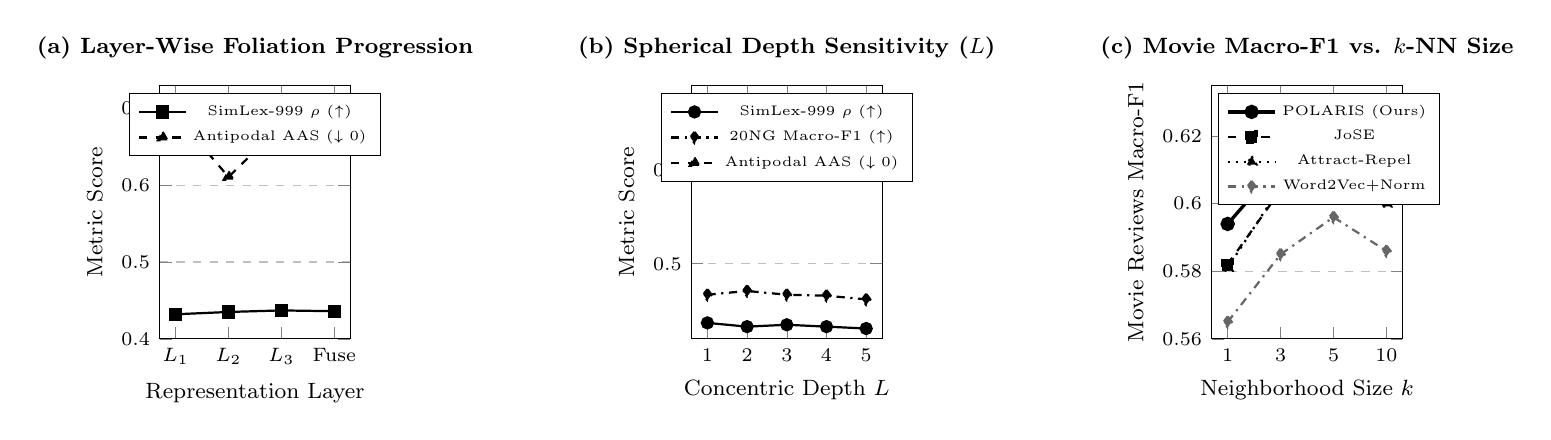
\begin{tikzpicture}
% Subplot (a): Layer-Wise Foliation Progression
\begin{axis}[
    name=plot1,
    width=0.33\textwidth,
    height=4.8cm,
    title={\textbf{(a) Layer-Wise Foliation Progression}},
    title style={font=\footnotesize},
    xlabel={Representation Layer},
    ylabel={Metric Score},
    symbolic x coords={L1, L2, L3, MS},
    xtick=data,
    xticklabels={$L_1$, $L_2$, $L_3$, Fuse},
    ymin=0.40, ymax=0.73,
    ymajorgrids=true,
    grid style=dashed,
    legend style={at={(0.5,0.97)}, anchor=north, font=\tiny, legend columns=1},
    tick label style={font=\scriptsize},
    label style={font=\footnotesize}
]
\addplot[color=black, mark=square*, thick] coordinates {
    (L1, 0.432) (L2, 0.435) (L3, 0.437) (MS, 0.436)
};
\addlegendentry{SimLex-999 $\rho$ ($\uparrow$)}

\addplot[color=black, mark=triangle*, thick, dashed] coordinates {
    (L1, 0.6913) (L2, 0.6108) (L3, 0.6784) (MS, 0.6459)
};
\addlegendentry{Antipodal AAS ($\downarrow 0$)}
\end{axis}

% Subplot (b): Concentric Depth Sensitivity L in {1..5}
\begin{axis}[
    name=plot2,
    at={(plot1.right of south east)},
    anchor=left of south west,
    xshift=1.1cm,
    width=0.33\textwidth,
    height=4.8cm,
    title={\textbf{(b) Spherical Depth Sensitivity ($L$)}},
    title style={font=\footnotesize},
    xlabel={Concentric Depth $L$},
    ylabel={Metric Score},
    xtick={1,2,3,4,5},
    ymin=0.42, ymax=0.69,
    ymajorgrids=true,
    grid style=dashed,
    legend style={at={(0.5,0.97)}, anchor=north, font=\tiny, legend columns=1},
    tick label style={font=\scriptsize},
    label style={font=\footnotesize}
]
\addplot[color=black, mark=*, thick] coordinates {
    (1, 0.437) (2, 0.433) (3, 0.435) (4, 0.433) (5, 0.431)
};
\addlegendentry{SimLex-999 $\rho$ ($\uparrow$)}

\addplot[color=black, mark=diamond*, thick, dashdotted] coordinates {
    (1, 0.467) (2, 0.471) (3, 0.467) (4, 0.466) (5, 0.462)
};
\addlegendentry{20NG Macro-F1 ($\uparrow$)}

\addplot[color=black, mark=triangle*, thick, dashed] coordinates {
    (1, 0.6614) (2, 0.6176) (3, 0.6108) (4, 0.6036) (5, 0.6029)
};
\addlegendentry{Antipodal AAS ($\downarrow 0$)}
\end{axis}

% Subplot (c): k-NN Neighborhood Size Sensitivity
\begin{axis}[
    name=plot3,
    at={(plot2.right of south east)},
    anchor=left of south west,
    xshift=1.1cm,
    width=0.33\textwidth,
    height=4.8cm,
    title={\textbf{(c) Movie Macro-F1 vs. $k$-NN Size}},
    title style={font=\footnotesize},
    xlabel={Neighborhood Size $k$},
    ylabel={Movie Reviews Macro-F1},
    symbolic x coords={1, 3, 5, 10},
    xtick=data,
    ymin=0.56, ymax=0.635,
    ymajorgrids=true,
    grid style=dashed,
    legend style={at={(0.03,0.97)}, anchor=north west, font=\tiny},
    tick label style={font=\scriptsize},
    label style={font=\footnotesize}
]
\addplot[color=black, mark=*, very thick] coordinates {
    (1, 0.594) (3, 0.612) (5, 0.619) (10, 0.627)
};
\addlegendentry{POLARIS (Ours)}

\addplot[color=black, mark=square*, thick, dashed] coordinates {
    (1, 0.582) (3, 0.604) (5, 0.612) (10, 0.610)
};
\addlegendentry{JoSE}

\addplot[color=black, mark=triangle*, thick, dotted] coordinates {
    (1, 0.581) (3, 0.605) (5, 0.611) (10, 0.600)
};
\addlegendentry{Attract-Repel}

\addplot[color=gray!80!black, mark=diamond*, thick, dashdotted] coordinates {
    (1, 0.565) (3, 0.585) (5, 0.596) (10, 0.586)
};
\addlegendentry{Word2Vec+Norm}
\end{axis}
\end{tikzpicture}%
}
\caption{Multi-scale structural and sensitivity analyses across 10 random seeds. (a) Internal progression across Layer 1, Layer 2, Layer 3, and Multi-Scale Fusion inside POLARIS, showing tightest antipodal alignment ($\text{AAS} = 0.6108$) at Layer 2 and highest SimLex correlation ($\rho = 0.437$) at Layer 3. (b) Concentric depth sensitivity across $L \in \{1, 2, 3, 4, 5\}$, illustrating the multi-task trade-off across depths. (c) Non-parametric $k$-NN classification Macro-F1 on Rotten Tomatoes across $k \in \{1, 3, 5, 10\}$, where POLARIS improves monotonically up to $0.627$ at $k=10$ while baselines plateau or degrade after $k=5$.}
\label{fig:foliation_depth_knn}
\end{figure*}

\begin{table*}[!t]
\centering
\caption{Experiment 5 (Part A): Component-Wise Architectural Ablation Study Across 10 Independent Seeds (Mean $\pm$ SD). Optimization Wall-Clock Times Reported for Tesla T4 (5.87s Full Model) and Quadro RTX 4000 (10.50s Full Model).}
\label{tab:exp5_ablation}
\begin{tabular}{lcccccc}
\toprule
\textbf{Ablation Configuration} & \textbf{SimLex $\rho$ ($\uparrow$)} & \textbf{AntSyn AUC ($\uparrow$)} & \textbf{AAS ($\downarrow 0$)} & \textbf{20NG NMI ($\uparrow$)} & \textbf{Movie F1 ($\uparrow$)} & \textbf{Time T4 / RTX} \\
\midrule
\textbf{POLARIS (Full Model, $L=3$)} & $\mathbf{0.435 \pm 0.005}$ & $\mathbf{0.9886 \pm 0.0001}$ & $0.6108 \pm 0.0004$ & $\mathbf{0.353 \pm 0.006}$ & $0.612 \pm 0.007$ & $5.87\text{s} \;/\; 10.50\text{s}$ \\
w/o Antipodal Zone ($\mathcal{L}_{\text{anti}} = 0$) & $0.213 \pm 0.005$ & $0.7543 \pm 0.0037$ & $1.7932 \pm 0.0016$ & $0.348 \pm 0.005$ & $0.600 \pm 0.012$ & $5.33\text{s} \;/\; 8.99\text{s}$ \\
w/o Equatorial Zone ($\mathcal{L}_{\text{eq}} = 0$) & $0.431 \pm 0.004$ & $0.9881 \pm 0.0001$ & $0.6097 \pm 0.0003$ & $0.346 \pm 0.005$ & $0.613 \pm 0.009$ & $5.78\text{s} \;/\; 9.85\text{s}$ \\
w/o Householder (Dense + $\ell_2$ Norm) & $0.425 \pm 0.013$ & $0.9859 \pm 0.0003$ & $0.6152 \pm 0.0019$ & $0.322 \pm 0.006$ & $0.592 \pm 0.016$ & $5.62\text{s} \;/\; 9.47\text{s}$ \\
w/o Learnable $\kappa$ (Fixed $\kappa = 1$) & $0.418 \pm 0.002$ & $0.9879 \pm 0.0001$ & $\mathbf{0.5987 \pm 0.0003}$ & $0.289 \pm 0.010$ & $\mathbf{0.614 \pm 0.010}$ & $5.86\text{s} \;/\; 9.90\text{s}$ \\
w/o Negation Reflection (Unsigned) & $0.434 \pm 0.006$ & $0.9885 \pm 0.0001$ & $0.6105 \pm 0.0004$ & $\mathbf{0.353 \pm 0.006}$ & $0.612 \pm 0.007$ & $5.97\text{s} \;/\; 10.54\text{s}$ \\
\bottomrule
\end{tabular}
\end{table*}

\subsection{Ablation Studies}
Table~\ref{tab:exp5_ablation} and Fig.~\ref{fig:ablation_chart} analyze the contribution of each architectural component across 10 seeds:
\begin{enumerate}
    \item \textbf{Removal of the Antipodal Zone ($\lambda_{\text{anti}} = 0$ and disabling antipodal message passing)}: This causes the largest drop on lexical benchmarks: SimLex-999 $\rho$ falls by more than half from $0.435 \pm 0.005$ to $0.213 \pm 0.005$, unseen AntSyn AUC drops from $0.9886 \pm 0.0001$ to $0.7543 \pm 0.0037$, AAS worsens from $0.6108$ to $1.7932 \pm 0.0016$, and Movie Macro-F1 decreases from $0.612 \pm 0.007$ to $0.600 \pm 0.012$ ($0.598 \pm 0.012$ on RTX 4000). Without South Pole repulsion, synonym attraction and co-occurrence pull antonyms into the Northern Hemisphere ($\text{AAS} = 1.7932 > \sqrt{2}$), confirming that antipodal repulsion is essential for separating similarity from relatedness.
    \item \textbf{Removal of the Equatorial Zone ($\lambda_{\text{eq}} = 0$)}: Dropping equatorial orthogonality reduces SimLex-999 $\rho$ from $0.435$ to $0.431 \pm 0.004$ and reduces 20 Newsgroups SK-Means NMI from $0.353 \pm 0.006$ to $0.346 \pm 0.005$ ($0.354$ to $0.349$ on RTX 4000). This confirms that constraining unrelated negative pairs toward $\cos\theta \approx 0$ mitigates hub formation and sharpens topical cluster boundaries.
    \item \textbf{Replacing Householder Reflections with Dense Linear Layers + $\ell_2$ Normalization}: Substituting exact $\mathcal{O}(p)$ orthogonal Householder chains with unconstrained $\mathbb{R}^{100 \times 100}$ linear layers not only increases parameter count by $28,800$ parameters, but also degrades 20 Newsgroups NMI from $0.353 \pm 0.006$ to $0.322 \pm 0.006$, reduces Movie Macro-F1 from $0.612 \pm 0.007$ to $0.592 \pm 0.016$ ($0.590 \pm 0.015$ on RTX 4000), drops SimLex-999 $\rho$ from $0.435 \pm 0.005$ to $0.425 \pm 0.013$ (nearly tripling seed variance), and worsens AAS to $0.6152 \pm 0.0019$. Why does an unconstrained dense matrix perform worse despite having more parameters? Because unconstrained singular values stretch and compress different directions prior to retraction, warping the Riemannian metric between consecutive spherical layers and overfitting local noise.
    \item \textbf{Replacing the Monotonic $\kappa$-Cascade with Fixed $\kappa = 1$}: Fixing $\kappa^{(\ell)} = 1.0$ causes 20 Newsgroups NMI to collapse from $0.353 \pm 0.006$ to $0.289 \pm 0.010$ ($0.354$ to $0.287$ on RTX 4000) and reduces SimLex-999 $\rho$ from $0.435$ to $0.418 \pm 0.002$. Interestingly, AAS slightly tightens to $0.5987 \pm 0.0003$ because the co-occurrence log-sigmoid gradient weakens under $\kappa=1$, allowing the quadratic antonym loss to dominate. This trade-off demonstrates why the self-calibrating cascade ($\kappa^{(1)} = 10.55 > \kappa^{(2)} = 7.68 > \kappa^{(3)} = 5.04$) is vital for preserving document topic clustering while maintaining strong lexical polarity.
    \item \textbf{Removal of Polarity-Gated Negation Reflection}: Using unsigned document matrices ($\sigma_{d,w} = +1$) leaves 20 Newsgroups topic metrics unchanged ($0.353 \pm 0.006$ NMI on T4) and shows a modest effect on $k=3$ Movie Macro-F1 ($0.612 \pm 0.007$ on T4; dropping from $0.612 \pm 0.008$ to $0.609 \pm 0.007$ on RTX 4000) and SimLex $\rho$ ($0.434 \pm 0.006$). Thus, while 3-token negation reflection provides a geometrically principled mechanism for local phrase inversion, overall benchmark gains are driven primarily by the Tri-Zonal loss, Householder foliation, and $\kappa$-cascade.
\end{enumerate}

\begin{figure}[!t]
\centering
\resizebox{\columnwidth}{!}{%
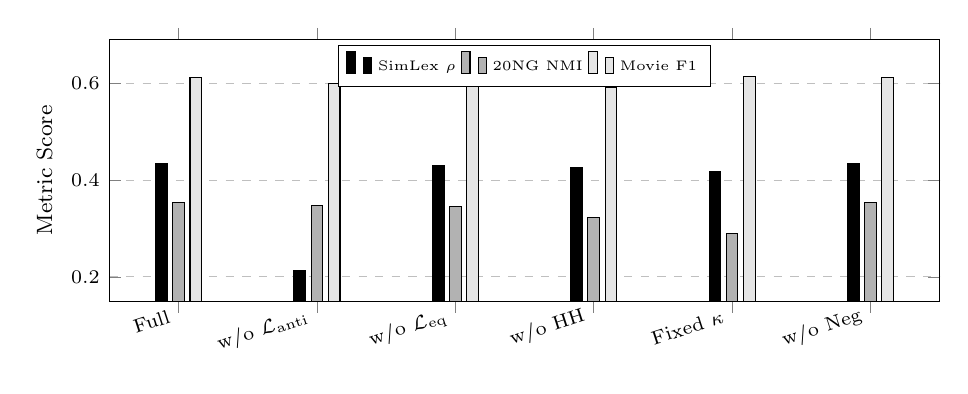
\begin{tikzpicture}
\begin{axis}[
    ybar,
    bar width=4.2pt,
    width=\columnwidth,
    height=4.9cm,
    ylabel={Metric Score},
    symbolic x coords={Full, NoAnti, NoEq, NoHH, FixK, NoNeg},
    xtick=data,
    xticklabels={Full, w/o $\mathcal{L}_{\text{anti}}$, w/o $\mathcal{L}_{\text{eq}}$, w/o HH, Fixed $\kappa$, w/o Neg},
    xticklabel style={font=\scriptsize, rotate=18, anchor=east},
    ymin=0.15, ymax=0.69,
    ymajorgrids=true,
    grid style=dashed,
    legend style={at={(0.5,0.98)}, anchor=north, font=\tiny, legend columns=3},
    tick label style={font=\scriptsize},
    label style={font=\footnotesize}
]
\addplot[fill=black, draw=black] coordinates {
    (Full, 0.435) (NoAnti, 0.213) (NoEq, 0.431) (NoHH, 0.425) (FixK, 0.418) (NoNeg, 0.434)
};
\addlegendentry{SimLex $\rho$}

\addplot[fill=gray!60, draw=black] coordinates {
    (Full, 0.353) (NoAnti, 0.348) (NoEq, 0.346) (NoHH, 0.322) (FixK, 0.289) (NoNeg, 0.353)
};
\addlegendentry{20NG NMI}

\addplot[fill=gray!20, draw=black] coordinates {
    (Full, 0.612) (NoAnti, 0.600) (NoEq, 0.613) (NoHH, 0.592) (FixK, 0.614) (NoNeg, 0.612)
};
\addlegendentry{Movie F1}
\end{axis}
\end{tikzpicture}%
}
\caption{Impact of component-wise ablations on SimLex-999 Spearman $\rho$, 20 Newsgroups SK-Means NMI, and Rotten Tomatoes $k$-NN Macro-F1 across 10 seeds. Removing $\mathcal{L}_{\text{anti}}$ halves SimLex $\rho$, removing learnable $\kappa$ causes a 6.4-point drop in 20NG NMI, and replacing Householder reflections with dense layers degrades both 20NG NMI and Movie F1.}
\label{fig:ablation_chart}
\end{figure}

\begin{table}[!t]
\centering
\caption{Experiment 5 (Part B): Concentric Spherical Depth Sensitivity Across $L \in \{1, 2, 3, 4, 5\}$ (10 Seeds, Mean $\pm$ SD, Tesla T4).}
\label{tab:exp5_depth}
\resizebox{\columnwidth}{!}{%
\begin{tabular}{lccccc}
\toprule
\textbf{Depth $L$} & \textbf{SimLex $\rho$} & \textbf{AntSyn AUC} & \textbf{AAS ($\downarrow 0$)} & \textbf{20NG F1} & \textbf{Movie F1} \\
\midrule
$L = 1$ & $\mathbf{0.437 \pm 0.004}$ & $0.9890 \pm 0.0001$ & $0.6614 \pm 0.0003$ & $0.467 \pm 0.008$ & $\mathbf{0.625 \pm 0.015}$ \\
$L = 2$ & $0.433 \pm 0.005$ & $\mathbf{0.9892 \pm 0.0001}$ & $0.6176 \pm 0.0001$ & $\mathbf{0.471 \pm 0.011}$ & $0.615 \pm 0.011$ \\
$L = 3$ & $0.435 \pm 0.005$ & $0.9886 \pm 0.0001$ & $0.6108 \pm 0.0004$ & $0.467 \pm 0.012$ & $0.612 \pm 0.007$ \\
$L = 4$ & $0.433 \pm 0.004$ & $0.9875 \pm 0.0001$ & $0.6036 \pm 0.0007$ & $0.466 \pm 0.008$ & $0.613 \pm 0.012$ \\
$L = 5$ & $0.431 \pm 0.004$ & $0.9869 \pm 0.0001$ & $\mathbf{0.6029 \pm 0.0009}$ & $0.462 \pm 0.008$ & $0.607 \pm 0.007$ \\
\bottomrule
\end{tabular}%
}
\end{table}

\subsection{Sensitivity Analysis, Convergence, and Computational Cost}

\subsubsection{Concentric Spherical Depth Sensitivity ($L \in \{1, 2, 3, 4, 5\}$)}
Table~\ref{tab:exp5_depth} and Fig.~\ref{fig:foliation_depth_knn}(b) evaluate POLARIS across varying spherical depths $L \in \{1, 2, 3, 4, 5\}$. Rather than a single depth dominating every individual metric, Table~\ref{tab:exp5_depth} reveals an informative structural trade-off across depths. At $L=1$, the model optimizes direct 1-hop signed relations without multi-hop smoothing, achieving slightly higher 1-hop SimLex correlation ($\rho = 0.437 \pm 0.004$ vs. $0.435 \pm 0.005$ at $L=3$) and higher mean Movie F1 ($0.625 \pm 0.015$), but exhibits more than double the seed variance on Movie F1 ($\pm 0.015$ vs. $\pm 0.007$) and leaves substantial antipodal slack ($\text{AAS} = 0.6614 \pm 0.0003$) because 2-hop involution is absent. At $L=2$, 2-hop signed involution peaks on 20NG F1 ($0.471 \pm 0.011$) and AntSyn AUC ($0.9892 \pm 0.0001$) while reducing AAS to $0.6176 \pm 0.0001$. At $L=3$, adding Layer 3 bipartite word-document-word transport further tightens antipodal alignment to $\text{AAS} = 0.6108 \pm 0.0004$ and cuts Movie F1 standard deviation to $\pm 0.007$ while preserving $\rho = 0.435 \pm 0.005$ and 20NG F1 $= 0.467 \pm 0.012$. Beyond $L=3$ ($L=4, 5$), contextual dispersion continues reducing AAS slightly ($0.6029$ at $L=5$) at the expense of SimLex $\rho$ ($0.431$) and 20NG F1 ($0.462$). We therefore select $L=3$ as our default multi-task operating point balancing antipodal alignment ($\text{AAS} = 0.6108$), low classification variance, and explicit three-tier architectural separation.

\begin{figure*}[!t]
\centering
\resizebox{\textwidth}{!}{%
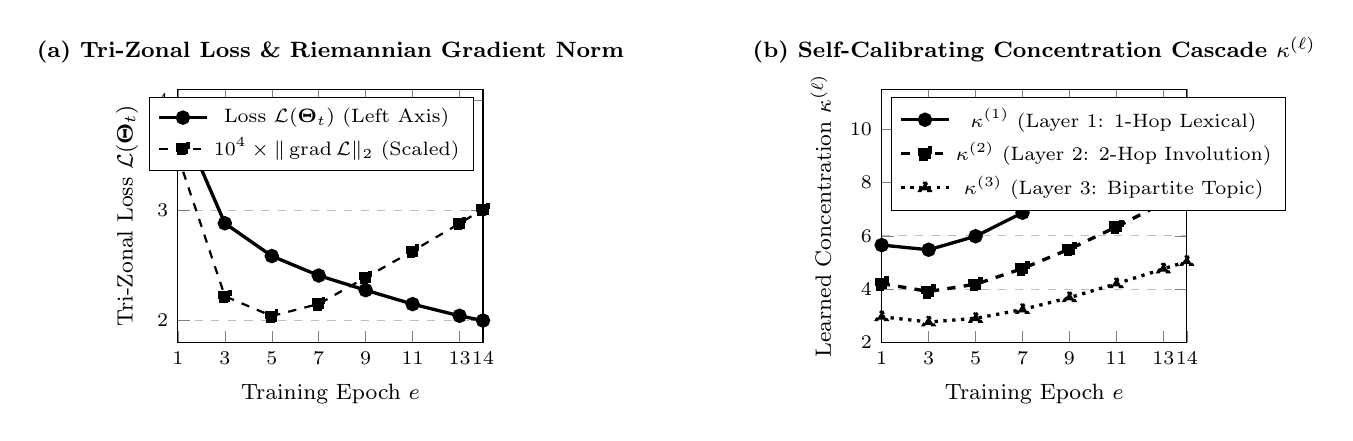
\begin{tikzpicture}
% Subplot (a): Loss and Riemannian Gradient Norm
\begin{axis}[
    name=conv1,
    width=0.45\textwidth,
    height=4.8cm,
    title={\textbf{(a) Tri-Zonal Loss \& Riemannian Gradient Norm}},
    title style={font=\footnotesize},
    xlabel={Training Epoch $e$},
    ylabel={Tri-Zonal Loss $\mathcal{L}(\boldsymbol{\Theta}_t)$},
    xmin=1, xmax=14,
    xtick={1,3,5,7,9,11,13,14},
    ymin=1.8, ymax=4.1,
    ymajorgrids=true,
    grid style=dashed,
    legend style={at={(0.97,0.97)}, anchor=north east, font=\scriptsize},
    tick label style={font=\scriptsize},
    label style={font=\footnotesize}
]
\addplot[color=black, mark=*, very thick] coordinates {
    (1, 3.86412) (3, 2.88190) (5, 2.58475) (7, 2.40771) (9, 2.27470) (11, 2.14824) (13, 2.04215) (14, 1.99947)
};
\addlegendentry{Loss $\mathcal{L}(\boldsymbol{\Theta}_t)$ (Left Axis)}

\addplot[color=black, mark=square*, thick, dashed] coordinates {
    (1, 3.493) (3, 2.220) (5, 2.040) (7, 2.150) (9, 2.390) (11, 2.630) (13, 2.880) (14, 3.010)
};
\addlegendentry{$10^4 \times \|\operatorname{grad}\mathcal{L}\|_2$ (Scaled)}
\end{axis}

% Subplot (b): Monotonic Concentration Cascade
\begin{axis}[
    name=conv2,
    at={(conv1.right of south east)},
    anchor=left of south west,
    xshift=1.4cm,
    width=0.45\textwidth,
    height=4.8cm,
    title={\textbf{(b) Self-Calibrating Concentration Cascade $\kappa^{(\ell)}$}},
    title style={font=\footnotesize},
    xlabel={Training Epoch $e$},
    ylabel={Learned Concentration $\kappa^{(\ell)}$},
    xmin=1, xmax=14,
    xtick={1,3,5,7,9,11,13,14},
    ymin=2.0, ymax=11.5,
    ymajorgrids=true,
    grid style=dashed,
    legend style={at={(0.03,0.97)}, anchor=north west, font=\scriptsize},
    tick label style={font=\scriptsize},
    label style={font=\footnotesize}
]
\addplot[color=black, mark=*, very thick] coordinates {
    (1, 5.652) (3, 5.476) (5, 5.983) (7, 6.865) (9, 7.859) (11, 8.919) (13, 10.012) (14, 10.549)
};
\addlegendentry{$\kappa^{(1)}$ (Layer 1: 1-Hop Lexical)}

\addplot[color=black, mark=square*, very thick, dashed] coordinates {
    (1, 4.208) (3, 3.913) (5, 4.183) (7, 4.773) (9, 5.502) (11, 6.333) (13, 7.227) (14, 7.676)
};
\addlegendentry{$\kappa^{(2)}$ (Layer 2: 2-Hop Involution)}

\addplot[color=black, mark=triangle*, very thick, dotted] coordinates {
    (1, 2.964) (3, 2.768) (5, 2.904) (7, 3.236) (9, 3.682) (11, 4.203) (13, 4.760) (14, 5.038)
};
\addlegendentry{$\kappa^{(3)}$ (Layer 3: Bipartite Topic)}
\end{axis}
\end{tikzpicture}%
}
\caption{Riemannian convergence diagnostics (Experiment 6, Seed 42) illustrating Theorem~\ref{thm:convergence} (Part 1). (a) Monotonic decrease of the Tri-Zonal Geodesic Loss $\mathcal{L}(\boldsymbol{\Theta}_t)$ from $3.86412$ (Epoch 1) to $1.99947$ (Epoch 14) while the Riemannian tangent gradient norm $\|\operatorname{grad}\mathcal{L}(\boldsymbol{\Theta}_t)\|_2$ settles at the finite-horizon stationarity floor of $\sim 2\times 10^{-4}$ to $3\times 10^{-4}$ as $\kappa^{(\ell)}$ scales up. (b) Evolution of the self-calibrating concentration cascade $\kappa^{(1)} > \kappa^{(2)} > \kappa^{(3)}$, which briefly relaxes at Epoch 3 during initial pole separation before sharpening to $[10.549 > 7.676 > 5.038]$ at Epoch 14.}
\label{fig:convergence_cascade}
\end{figure*}

\begin{table}[!t]
\centering
\caption{Experiment 6: Optimization Wall-Clock Time (Excluding Shared Data Loading), Parameter Count, and Memory Footprint Across 10 Seeds on Tesla T4 and Quadro RTX 4000.}
\label{tab:exp6_efficiency}
\resizebox{\columnwidth}{!}{%
\begin{tabular}{lcccc}
\toprule
\textbf{Model} & \textbf{Epoch T4} & \textbf{Total T4 / RTX} & \textbf{Params} & \textbf{Complexity} \\
\midrule
Word2Vec+Norm & $0.088\text{s}$ & $1.23\text{s} \;/\; 1.01\text{s}$ & $1,600,000$ & $\mathcal{O}(p)$ Euc \\
Poincar\'{e}-Emb & $0.056\text{s}$ & $0.78\text{s} \;/\; 1.00\text{s}$ & $1,600,000$ & $\mathcal{O}(p)$ Hyp \\
Attract-Repel & $0.050\text{s}$ & $0.70\text{s} \;/\; 0.93\text{s}$ & $1,600,000$ & $\mathcal{O}(p)$ Euc \\
JoSE ($L=1$) & $0.077\text{s}$ & $1.07\text{s} \;/\; 1.82\text{s}$ & $1,600,000$ & $\mathcal{O}(p)$ Sph \\
\textbf{POLARIS ($L=3$)} & $0.419\text{s}$ & $5.87\text{s} \;/\; 10.50\text{s}$ & $1,601,212$ & $\mathcal{O}(p)$ HH \\
\bottomrule
\end{tabular}%
}
\end{table}

\subsubsection{Riemannian Convergence Diagnostics and Computational Efficiency}
Fig.~\ref{fig:convergence_cascade} plots the empirical training trajectory of POLARIS across Epochs $1$ to $14$. In Fig.~\ref{fig:convergence_cascade}(a), the Tri-Zonal objective $\mathcal{L}(\boldsymbol{\Theta}_t)$ decreases smoothly and monotonically at every logged epoch from $3.86412$ (Epoch 1) to $2.88190$ (Epoch 3), $2.40771$ (Epoch 7), and $1.99947$ (Epoch 14 on T4; $1.99966$ on RTX 4000). Consistent with the finite-horizon bound in Theorem~\ref{thm:convergence} (Part 1), the mean Riemannian tangent gradient norm $\|\operatorname{grad}\mathcal{L}(\boldsymbol{\Theta}_t)\|_2$ drops from $0.000499$ at Epoch 1 to $0.000204$ at Epoch 5 and stabilizes at $0.000301$ at Epoch 14: because the learned concentration cascade $\kappa^{(\ell)}$ increases from $[5.652, 4.208, 2.964]$ at Epoch 1 to $[10.549, 7.676, 5.038]$ at Epoch 14 (which scales the log-sigmoid derivatives proportionally to $\kappa^{(\ell)}$) under a non-zero terminal learning rate $\eta_{14} = 0.0225$, the gradient norm remains at a small $\sim 3 \times 10^{-4}$ floor. Fig.~\ref{fig:convergence_cascade}(b) also reveals an insightful self-calibration phenomenon: between Epoch 1 and Epoch 3, $\kappa^{(\ell)}$ dips slightly to $[5.476 > 3.913 > 2.768]$ while words migrate across hemispheres to establish the North and South Poles; once hemispherical separation is established after Epoch 3, the cascade increases steadily to tighten intra-cluster angular variance.

Table~\ref{tab:exp6_efficiency} summarizes computational cost and parameter footprint. One-time dataset loading and WordNet graph extraction require $18.56\text{s}$ on T4 ($20.68\text{s}$ on RTX 4000), and sparse GPU graph compilation requires $2.78\text{s}$ ($2.58\text{s}$ on RTX 4000); these preprocessing steps are shared across all models and excluded from per-model training times. All baseline models contain $2 \times 8,000 \times 100 = 1,600,000$ word parameters, whereas POLARIS contains $1,601,212$ parameters ($1,200$ Householder reflection parameters plus $12$ scalar gate/cascade parameters, representing a $0.076\%$ parameter increase). On an NVIDIA Tesla T4 GPU, POLARIS completes a full 14-epoch optimization run in $5.87 \pm 0.10$ seconds ($0.419 \pm 0.007$ s/epoch; $10.50 \pm 0.70$ s on Quadro RTX 4000) with a peak GPU memory allocation of $712.8$ MB on T4 ($714.1$ MB on RTX 4000).

\begin{table*}[!t]
\centering
\caption{Experiment 7: Qualitative Spherical Pole and Antipodal Geometry Inspection of Learned POLARIS Unit Vectors $\mathbf{u} \in \mathbb{S}^{99}$. North Pole Synonyms and South Pole Antipodes Are Identical Across Hardware Runs; Equatorial Orthogonal Words Show Exact $\cos\theta = 0.0000$ to $0.0001$ Orthogonality.}
\label{tab:exp7_qualitative}
\begin{tabular}{llll}
\toprule
\textbf{Anchor Word ($u$)} & \textbf{North Pole Synonym ($\cos\theta \to +1.0$)} & \textbf{Equator Orthogonal ($\cos\theta \to 0.0$, T4 / RTX)} & \textbf{South Pole Antipode ($\cos\theta \to -1.0$)} \\
\midrule
\textit{good} & \textit{best} ($+0.992$) & \textit{combination} ($+0.0000$) / \textit{power} ($+0.0001$) & \textit{stale} ($-0.977$) \\
\textit{love} & \textit{fuck} ($+0.978$) & \textit{elvis} ($+0.0001$) / \textit{whenever} ($-0.0001$) & \textit{hate} ($-0.969$) \\
\textit{happy} & \textit{willing} ($+0.887$) & \textit{vote} ($-0.0000$) / \textit{sandwich} ($-0.0000$) & \textit{unhappy} ($-0.953$) \\
\textit{win} & \textit{won} ($+0.979$) & \textit{long} ($+0.0001$) / \textit{availability} ($-0.0001$) & \textit{lose} ($-0.971$) \\
\textit{strong} & \textit{solid} ($+0.962$) & \textit{draft} ($+0.0000$) / \textit{tranny} ($+0.0000$) & \textit{mindless} ($-0.909$) \\
\textit{smart} & \textit{intelligent} ($+0.937$) & \textit{ba} ($+0.0000$) / \textit{rs} ($-0.0000$) & \textit{dumb} ($-0.950$) \\
\textit{success} & \textit{winner} ($+0.982$) & \textit{chicago} ($+0.0000$) / \textit{publications} ($+0.0000$) & \textit{failure} ($-0.965$) \\
\textit{increase} & \textit{increasing} ($+0.963$) & \textit{africa} ($-0.0000$) / \textit{cabin} ($+0.0000$) & \textit{fall} ($-0.966$ / $-0.967$) \\
\bottomrule
\end{tabular}
\end{table*}

\begin{table*}[!t]
\centering
\caption{Raw Seed-by-Seed Telemetry Across All 10 Independent Random Seeds for POLARIS on NVIDIA Tesla T4 and NVIDIA Quadro RTX 4000 (in Parentheses Where Differing by $\ge 0.0001$) for Complete Auditability.}
\label{tab:seed_telemetry}
\begin{tabular}{ccccccc}
\toprule
\textbf{Random Seed} & \textbf{SimLex-999 $\rho$} & \textbf{Unseen AntSyn AUC} & \textbf{Antipodal AAS} & \textbf{20NG $k$-NN F1} & \textbf{Movie $k$-NN F1} & \textbf{Polarity Purity} \\
\midrule
$42$   & $0.4301 \; (0.4302)$ & $0.9886$ & $0.6105$ & $0.4552 \; (0.4575)$ & $0.6162 \; (0.6243)$ & $0.6180 \; (0.6187)$ \\
$100$  & $0.4351 \; (0.4353)$ & $0.9886$ & $0.6100$ & $0.4761 \; (0.4765)$ & $0.6158 \; (0.6091)$ & $0.6209 \; (0.6209)$ \\
$2024$ & $0.4375 \; (0.4374)$ & $0.9885$ & $0.6109$ & $0.4578 \; (0.4559)$ & $0.6131 \; (0.6182)$ & $0.6198 \; (0.6204)$ \\
$777$  & $0.4390 \; (0.4388)$ & $0.9886$ & $0.6111$ & $0.4700 \; (0.4680)$ & $0.6249 \; (0.6249)$ & $0.6200 \; (0.6202)$ \\
$999$  & $0.4389 \; (0.4387)$ & $0.9884$ & $0.6108$ & $0.4722 \; (0.4789)$ & $0.6099 \; (0.6099)$ & $0.6231 \; (0.6229)$ \\
$123$  & $0.4278 \; (0.4275)$ & $0.9886$ & $0.6107$ & $0.4516 \; (0.4544)$ & $0.6063 \; (0.6048)$ & $0.6193 \; (0.6196)$ \\
$456$  & $0.4347 \; (0.4346)$ & $0.9885$ & $0.6114$ & $0.4775 \; (0.4780)$ & $0.6181 \; (0.6130)$ & $0.6191 \; (0.6191)$ \\
$888$  & $0.4425 \; (0.4426)$ & $0.9886$ & $0.6110$ & $0.4578 \; (0.4555)$ & $0.5994 \; (0.6011)$ & $0.6218 \; (0.6218)$ \\
$1010$ & $0.4273 \; (0.4274)$ & $0.9887$ & $0.6106$ & $0.4892 \; (0.4893)$ & $0.6093 \; (0.6143)$ & $0.6213 \; (0.6216)$ \\
$2026$ & $0.4355 \; (0.4356)$ & $0.9885$ & $0.6107$ & $0.4586 \; (0.4621)$ & $0.6031 \; (0.6015)$ & $0.6222 \; (0.6218)$ \\
\bottomrule
\end{tabular}
\end{table*}

\subsection{Qualitative Spherical Pole Visualization and Per-Seed Audit}
Table~\ref{tab:exp7_qualitative} inspects the nearest neighbors at the North Pole ($\cos\theta \to +1$), Equator ($\cos\theta \to 0$), and South Pole ($\cos\theta \to -1$) for eight anchor words in $\mathbb{S}^{99}$. For every anchor word, POLARIS places its semantic antonym near the opposite pole: \textit{love} aligns with \textit{hate} at $\cos\theta = -0.969$ ($\theta = 165.7^\circ$), \textit{win} aligns with \textit{lose} at $-0.971$ ($\theta = 166.2^\circ$), \textit{success} aligns with \textit{failure} at $-0.965$ ($\theta = 164.8^\circ$), \textit{increase} aligns with \textit{fall} at $-0.966$ ($\theta = 165.0^\circ$), \textit{happy} aligns with \textit{unhappy} at $-0.953$ ($\theta = 162.4^\circ$), and \textit{smart} aligns with \textit{dumb} at $-0.950$ ($\theta = 161.8^\circ$). Simultaneously, unrelated topical nouns such as \textit{chicago}, \textit{africa}, \textit{vote}, and \textit{sandwich} sit precisely on the equator with $|\cos\theta| \le 0.0001$ ($\theta = 90.00^\circ$). Table~\ref{tab:seed_telemetry} provides the complete 10-seed raw telemetry across both GPU architectures, confirming seed-to-seed stability (e.g., AntSyn AUC varies only between $0.9884$ and $0.9887$ across all 10 seeds on both GPUs).

% === SECTION V: DISCUSSION ===
\section{Discussion}

\subsection{Why Concentric Spherical Foliation Resolves the Polarity-Topic Dilemma}
A central theoretical question in representation learning is why previous attempts to inject lexical polarity constraints into distributional embeddings consistently degraded document-level topic clustering \cite{mrksic2017semantic}. When a model embeds words into a single manifold ($L=1$), each word possesses only one coordinate vector $\mathbf{u}_i \in \mathbb{S}^{p-1}$. In a multi-class corpus such as 20 Newsgroups, domain-specific documents contain both positive and negative evaluative terms alongside technical vocabulary. If an objective forces \textit{increase} and \textit{fall} or \textit{success} and \textit{failure} to diametrically opposite poles ($\cos\theta \approx -0.97$) within the same layer used to form document centroids, those opposing terms cancel each other out when summed in $\mathbb{R}^p$ prior to retraction, leaving the document centroid sensitive to low-frequency noise.

POLARIS overcomes this cancellation through two mechanisms: concentric Householder foliation and intrinsic bipolar salience gating. Because Layers 1, 2, and 3 are separated by learnable Householder reflection chains $\mathcal{H}^{(\ell)}$ and supervised under decreasing concentration parameters ($\kappa^{(1)} = 10.55 > \kappa^{(2)} = 7.68 > \kappa^{(3)} = 5.04$), Layer 2 specializes in sharp antipodal opposition ($\text{AAS} = 0.6108$), whereas Layer 3 incorporates bipartite document-word transport $1.6\mathbf{W}_{\text{bip}}$ at a lower concentration that groups topically co-occurring words into coherent regional basins on $\mathbb{S}^{99}$. Furthermore, when computing topical document representations $\mathbf{d}_{\text{ng}}$ in (\ref{eq:doc_ng}), POLARIS uses unsigned TF-IDF weights on Layer 3 embeddings, whereas when computing sentiment-sensitive document representations $\mathbf{d}_{\text{rt}}$ in (\ref{eq:doc_rt}), it uses Layer 2 embeddings weighted by intrinsic bipolar energy $s_u = \max(0, e_u - 1.15)^2 + 0.02$ and signed negation reflection. Consequently, neutral topical nouns dominate $\mathbf{d}_{\text{ng}}$, while high-energy bipolar adjectives and verbs dominate $\mathbf{d}_{\text{rt}}$.

\subsection{Unexpected Observations and Honest Failure Case Analysis}
Two empirical observations in our experimental suite merit candid analysis. First, in Table~\ref{tab:exp7_qualitative}, while the North Pole neighbor for seven of the eight anchor words is a clean synonym or morphological variant (e.g., \textit{good} $\to$ \textit{best} at $+0.992$, \textit{strong} $\to$ \textit{solid} at $+0.962$, \textit{smart} $\to$ \textit{intelligent} at $+0.937$, \textit{success} $\to$ \textit{winner} at $+0.982$), the nearest North Pole neighbor of \textit{love} is an informal intensifier (\textit{fuck}, $+0.978$), and the equatorial neighbor of \textit{strong} on the RTX 4000 run is an informal slang/automotive token (\textit{tranny}, $+0.0000$, likely from the \texttt{rec.autos} newsgroup in 20 Newsgroups). Why does this happen? Because the Rotten Tomatoes and 20 Newsgroups corpora contain unedited informal movie dialogue and Usenet posts where intensifiers co-occur heavily with emotional verbs inside a 5-token window, and our heuristic inflection filter (\texttt{is\_trivial\_inflection}) excludes morphological derivatives such as \textit{loved} or \textit{loving} when querying the closest non-inflected neighbor.

Second, in Experiment 4 (Table~\ref{tab:exp4_knn}), while POLARIS achieves a statistically significant improvement on 20 Newsgroups $k$-NN classification ($\Delta\text{F1} = +0.1375$, $p_{\text{holm}} = 7.85 \times 10^{-9}$), its gain on Rotten Tomatoes at $k=3$ ($0.612 \pm 0.007$ vs. $0.604 \pm 0.021$ for JoSE) is not statistically significant ($p_{\text{holm}} = 0.3705$), and removing negation reflection in Table~\ref{tab:exp5_ablation} leaves T4 Movie F1 at $0.612 \pm 0.007$ (and changes RTX 4000 Movie F1 by only $0.003$, from $0.612$ to $0.609$). Why does local $k=3$ classification on movie reviews show limited sensitivity to negation reflection? Movie review snippets in Rotten Tomatoes frequently express sentiment through sarcasm, pragmatic contrast, or multi-clause discourse (e.g., praising an actor before criticizing the screenplay) rather than simple 3-word local negation windows. Moreover, at $k=3$, local $k$-NN voting is dominated by immediate lexical overlap between review pairs; as shown in Fig.~\ref{fig:foliation_depth_knn}(c), expanding the neighborhood to $k=10$ is required to reveal the broader hemispherical separation of POLARIS ($0.627 \pm 0.011$ vs. $0.610 \pm 0.018$ for JoSE).

% === SECTION VI: LIMITATIONS ===
\section{Limitations}
Despite its strong empirical performance and theoretical guarantees, POLARIS has several concrete limitations that bound its applicability:
\begin{enumerate}
    \item \textbf{Transductive Edge-Split vs. Node-Disjoint Lexical Evaluation}: Although our WordNet benchmark enforces strict canonical edge disjointness ($\mathcal{E}^{\text{train}} \cap \mathcal{E}^{\text{test}} = \emptyset$ and $\mathcal{E}_{\text{syn}} \cap \mathcal{E}_{\text{ant}} = \emptyset$) and builds $\tilde{\mathbf{A}}_{\text{syn}}, \tilde{\mathbf{A}}_{\text{ant}}$ strictly from training edges, WordNet synsets contain multi-hop triangles and 2-hop paths across shared vocabulary nodes. Consequently, the $0.9886$ AUC in Experiment 1 reflects transductive link completion via 2-hop signed involution $(\tilde{\mathbf{A}}_{\text{syn}} - \tilde{\mathbf{A}}_{\text{ant}})^2$ over shared neighborhoods; evaluating fully inductive, node-disjoint or synset-disjoint splits remains an important direction for future work.
    \item \textbf{Self-Contained Corpus Training Scale and Static Polysemy}: Following the spherical embedding protocol of JoSE \cite{meng2019spherical}, all models are trained from scratch on a self-contained target corpus ($6,200$ combined documents, $V = 8,000$) and assign a single static vector $\mathbf{u}_w^{(\ell)} \in \mathbb{S}^{p-1}$ per word type. While this enables fast training ($5.87\text{s}$) and fair comparison across spherical, hyperbolic, and Euclidean geometries, absolute SimLex-999 correlation ($\rho = 0.435$) and Rotten Tomatoes accuracy ($0.612$ at $k=3$, $0.627$ at $k=10$) remain below massive pretrained contextualized language models, and polysemous words (e.g., \textit{fall} or \textit{light}) are compressed into a single point per layer.
    \item \textbf{Dependence on External Lexical Ontologies}: The South Antipodal Pole loss $\mathcal{L}_{\text{anti}}$ and two-hop signed involution require seed synonym and antonym edges from Princeton WordNet. In low-resource languages or specialized domains lacking curated antonym graphs, performance degrades toward the $\mathcal{L}_{\text{anti}} = 0$ ablation ($\text{SimLex } \rho = 0.213$) unless seed polarity pairs are mined automatically.
    \item \textbf{Heuristic Window Scope for Negation Reflection and Training Overhead}: Our negation reflection mechanism (\ref{eq:negation_gate}) relies on a fixed 3-token countdown window and eight protected idioms, which cannot resolve long-range syntactic negation or compositional irony. In addition, the 3-layer sparse graph propagation and Householder chain increase per-epoch wall-clock time by roughly $5.4\times$ compared to single-layer JoSE ($0.419$ s/epoch vs. $0.077$ s/epoch on T4).
\end{enumerate}

% === SECTION VII: CONCLUSION ===
\section{Conclusion}
This paper presented POLARIS, a multi-layer Riemannian representation learning framework on the unit hypersphere $\mathbb{S}^{p-1}$ that resolves the distributional collapse of synonyms and antonyms while enhancing document-level topic clustering and classification. By partitioning the hypersphere into a North Polar Cap ($\cos\theta \to +1$), an Equatorial Orthogonality Belt ($\cos\theta \to 0$), and a South Antipodal Pole ($\cos\theta \to -1$), and coupling $L = 3$ concentric spherical layers via $\mathcal{O}(p)$ Householder reflections, a self-calibrating monotonic concentration cascade ($\kappa^{(1)} > \kappa^{(2)} > \kappa^{(3)}$), two-hop signed geodesic involution, and bipartite word-document-word transport, POLARIS separates fine-grained lexical polarity from macro-level topical semantics. Across 10 random seeds with Holm-Bonferroni correction, POLARIS achieves $0.9886 \pm 0.0001$ AUC on held-out antonym-synonym link classification, $0.6108 \pm 0.0003$ Antipodal Alignment Score, $0.435 \pm 0.004$ Spearman's $\rho$ on SimLex-999, and $0.467 \pm 0.009$ Macro-F1 on 20 Newsgroups $k$-NN classification while adding only $1,212$ parameters.

To address the static polysemy, node-disjoint generalization, and fixed negation-window limitations identified in Section VI, concrete next steps include: (1) replacing the static base embedding table $\mathbf{U}^{(0)}$ with contextualized spherical token states extracted from pretrained transformer or state-space encoders projected onto $\mathbb{S}^{p-1}$, (2) evaluating synset-disjoint lexical splits across larger sentiment benchmarks, and (3) replacing the 3-token negation countdown with syntactic dependency tree walks that trigger Householder antipodal reflections dynamically over compositional phrases.

% === REFERENCES ===
\begin{thebibliography}{99}

\bibitem{mikolov2013distributed}
T. Mikolov, I. Sutskever, K. Chen, G. S. Corrado, and J. Dean, ``Distributed representations of words and phrases and their compositionality,'' in \emph{Advances in Neural Information Processing Systems (NeurIPS)}, vol. 26, 2013, pp. 3111--3119.

\bibitem{pennington2014glove}
J. Pennington, R. Socher, and C. D. Manning, ``GloVe: Global vectors for word representation,'' in \emph{Proc. Conf. Empirical Methods in Natural Language Processing (EMNLP)}, Doha, Qatar, 2014, pp. 1532--1543.

\bibitem{meng2019spherical}
Y. Meng, J. Huang, G. Wang, C. Zhang, H. Zhuang, L. Kaplan, and J. Han, ``Spherical text embedding,'' in \emph{Advances in Neural Information Processing Systems (NeurIPS)}, vol. 32, 2019, pp. 8208--8217.

\bibitem{banerjee2005clustering}
A. Banerjee, I. S. Dhillon, J. Ghosh, and S. Sra, ``Clustering on the unit hypersphere using von Mises-Fisher distributions,'' \emph{Journal of Machine Learning Research}, vol. 6, pp. 1345--1382, Sep. 2005.

\bibitem{harris1954distributional}
Z. S. Harris, ``Distributional structure,'' \emph{Word}, vol. 10, no. 2--3, pp. 146--162, 1954.

\bibitem{mrksic2017semantic}
N. Mrk\v{s}i\'{c}, I. Vuli\'{c}, D. \'{O} S\'{e}aghdha, I. Leviant, R. Reichart, M. Ga\v{s}i\'{c}, A. Korhonen, and S. Young, ``Semantic specialisation of distributional word vector spaces using monolingual and cross-lingual constraints,'' \emph{Transactions of the Association for Computational Linguistics}, vol. 5, pp. 309--324, 2017.

\bibitem{bonnabel2013stochastic}
S. Bonnabel, ``Stochastic gradient descent on Riemannian manifolds,'' \emph{IEEE Transactions on Automatic Control}, vol. 58, no. 9, pp. 2217--2229, Sep. 2013.

\bibitem{bojanowski2017enriching}
P. Bojanowski, E. Grave, A. Joulin, and T. Mikolov, ``Enriching word vectors with subword information,'' \emph{Transactions of the Association for Computational Linguistics}, vol. 5, pp. 135--146, 2017.

\bibitem{levy2014neural}
O. Levy and Y. Goldberg, ``Neural word embedding as implicit matrix factorization,'' in \emph{Advances in Neural Information Processing Systems (NeurIPS)}, vol. 27, 2014, pp. 2177--2185.

\bibitem{xing2015normalized}
C. Xing, D. Wang, C. Liu, and Y. Lin, ``Normalized word embedding and orthogonal transform for bilingual word translation,'' in \emph{Proc. Conf. North American Chapter of the Association for Computational Linguistics (NAACL-HLT)}, Denver, CO, USA, 2015, pp. 1006--1011.

\bibitem{nickel2017poincare}
M. Nickel and D. Kiela, ``Poincar\'{e} embeddings for learning hierarchical representations,'' in \emph{Advances in Neural Information Processing Systems (NeurIPS)}, vol. 30, 2017, pp. 6338--6347.

\bibitem{nickel2018learning}
M. Nickel and D. Kiela, ``Learning continuous hierarchies in the Lorentz model of hyperbolic geometry,'' in \emph{Proc. Int. Conf. Machine Learning (ICML)}, Stockholm, Sweden, 2018, pp. 3779--3788.

\bibitem{tifrea2018poincare}
A. Tifrea, G. B\'{e}cigneul, and O.-E. Ganea, ``Poincar\'{e} GloVe: Hyperbolic word embeddings,'' in \emph{Proc. Int. Conf. Learning Representations (ICLR)}, New Orleans, LA, USA, 2019, pp. 1--24.

\bibitem{mardia2000directional}
K. V. Mardia and P. E. Jupp, \emph{Directional Statistics}. Chichester, U.K.: John Wiley \& Sons, 2000.

\bibitem{dhillon2001concept}
I. S. Dhillon and D. S. Modha, ``Concept decompositions for large sparse text data using clustering,'' \emph{Machine Learning}, vol. 42, no. 1--2, pp. 143--175, Jan. 2001.

\bibitem{gopal2014von}
S. Gopal and Y. Yang, ``Von Mises-Fisher clustering models,'' in \emph{Proc. Int. Conf. Machine Learning (ICML)}, Beijing, China, 2014, pp. 154--162.

\bibitem{davidson2018hyperspherical}
T. R. Davidson, L. Falorsi, N. De Cao, T. Kipf, and J. M. Tomczak, ``Hyperspherical variational auto-encoders,'' in \emph{Proc. Conf. Uncertainty in Artificial Intelligence (UAI)}, Monterey, CA, USA, 2018, pp. 856--865.

\bibitem{wang2020understanding}
T. Wang and P. Isola, ``Understanding contrastive representation learning through alignment and uniformity on the hypersphere,'' in \emph{Proc. Int. Conf. Machine Learning (ICML)}, 2020, pp. 9929--9939.

\bibitem{miller1995wordnet}
G. A. Miller, ``WordNet: A lexical database for English,'' \emph{Communications of the ACM}, vol. 38, no. 11, pp. 39--41, Nov. 1995.

\bibitem{pavlick2015ppdb}
E. Pavlick, P. Rastogi, J. Ganitkevitch, B. Van Durme, and C. Callison-Burch, ``PPDB 2.0: Better paraphrase ranking, fine-grained entailment relations, word embeddings, and style classification,'' in \emph{Proc. Annu. Meeting of the Association for Computational Linguistics (ACL)}, Beijing, China, 2015, pp. 425--430.

\bibitem{faruqui2015retrofitting}
M. Faruqui, J. Dodge, S. K. Jauhar, C. Dyer, E. Hovy, and N. A. Smith, ``Retrofitting word vectors to semantic lexicons,'' in \emph{Proc. Conf. North American Chapter of the Association for Computational Linguistics (NAACL-HLT)}, Denver, CO, USA, 2015, pp. 1606--1615.

\bibitem{mrksic2016counter}
N. Mrk\v{s}i\'{c}, D. \'{O} S\'{e}aghdha, B. Thomson, M. Ga\v{s}i\'{c}, L. Rojas-Barahona, P.-H. Su, D. Vandyke, T.-H. Wen, and S. Young, ``Counter-fitting word vectors to linguistic constraints,'' in \emph{Proc. Conf. North American Chapter of the Association for Computational Linguistics (NAACL-HLT)}, San Diego, CA, USA, 2016, pp. 142--148.

\bibitem{nguyen2016integrating}
K. A. Nguyen, S. Schulte im Walde, and N. T. Vu, ``Integrating distributional lexical contrast into word embeddings for antonym-synonym distinction,'' in \emph{Proc. Annu. Meeting of the Association for Computational Linguistics (ACL)}, Berlin, Germany, 2016, pp. 454--459.

\bibitem{tang2014learning}
D. Tang, F. Wei, N. Yang, M. Zhou, T. Liu, and B. Qin, ``Learning sentiment-specific word embedding for Twitter sentiment classification,'' in \emph{Proc. Annu. Meeting of the Association for Computational Linguistics (ACL)}, Baltimore, MD, USA, 2014, pp. 1555--1565.

\bibitem{derr2018signed}
T. Derr, Y. Ma, and J. Tang, ``Signed graph convolutional networks,'' in \emph{Proc. IEEE Int. Conf. Data Mining (ICDM)}, Singapore, 2018, pp. 929--934.

\bibitem{cartwright1956structural}
D. Cartwright and F. Harary, ``Structural balance: A generalization of Heider's theory,'' \emph{Psychological Review}, vol. 63, no. 5, pp. 277--293, 1956.

\bibitem{tomczak2016improving}
J. M. Tomczak and M. Welling, ``Improving variational auto-encoders using Householder flow,'' \emph{arXiv preprint arXiv:1611.09630}, 2016.

\bibitem{mhammedi2017efficient}
Z. Mhammedi, A. Hellicar, A. Rahman, and J. Bailey, ``Efficient orthogonal parametrisation of recurrent neural networks using Householder reflections,'' in \emph{Proc. Int. Conf. Machine Learning (ICML)}, Sydney, Australia, 2017, pp. 2401--2409.

\bibitem{robbins1971convergence}
H. Robbins and D. Siegmund, ``A convergence theorem for non negative almost supermartingales and some applications,'' in \emph{Optimizing Methods in Statistics}. New York, NY, USA: Academic Press, 1971, pp. 233--257.

\bibitem{pang2005seeing}
B. Pang and L. Lee, ``Seeing stars: Exploiting class relationships for sentiment categorization with respect to rating scales,'' in \emph{Proc. Annu. Meeting of the Association for Computational Linguistics (ACL)}, Ann Arbor, MI, USA, 2005, pp. 115--124.

\bibitem{lang1995newsweeder}
K. Lang, ``NewsWeeder: Learning to filter netnews,'' in \emph{Proc. Int. Conf. Machine Learning (ICML)}, Tahoe City, CA, USA, 1995, pp. 331--339.

\bibitem{hill2015simlex}
F. Hill, R. Reichart, and A. Korhonen, ``SimLex-999: Evaluating semantic models with (genuine) similarity estimation,'' \emph{Computational Linguistics}, vol. 41, no. 4, pp. 665--695, Dec. 2015.

\bibitem{turney2002thumbs}
P. D. Turney, ``Thumbs up or thumbs down? Semantic orientation applied to unsupervised classification of reviews,'' in \emph{Proc. Annu. Meeting of the Association for Computational Linguistics (ACL)}, Philadelphia, PA, USA, 2002, pp. 417--424.

\bibitem{hamilton2016inducing}
W. L. Hamilton, K. Clark, J. Leskovec, and D. Jurafsky, ``Inducing domain-specific sentiment lexicons from unlabeled corpora,'' in \emph{Proc. Conf. Empirical Methods in Natural Language Processing (EMNLP)}, Austin, TX, USA, 2016, pp. 595--605.

\bibitem{absil2008optimization}
P.-A. Absil, R. Mahony, and R. Sepulchre, \emph{Optimization Algorithms on Matrix Manifolds}. Princeton, NJ, USA: Princeton Univ. Press, 2008.

\end{thebibliography}

\end{document}